% Choose a font that is clearly legible and appropriate for a research paper. The font size
% should appear on the page at least as large as Times New Roman 11pt font. Captions
% may be smaller if legible.
% Use 1.5 line spacing and 1” margins on all sides. Do not use multiple columns. 

\documentclass[11pt]{article}
\usepackage[left=1in,right=1in,top=1in,bottom=1in]{geometry}
\usepackage[moderate]{savetrees} % I think this messes with the linespread thing...
\linespread{1.25} % THIS MULTIPLIES the skip factor, which defaults to 1.2 in LaTex, by 1.25, thus making the line spacing 1.5

\newcommand{\note}[1]{\textcolor{red}{#1}}

\usepackage{algorithm, algpseudocode}

\usepackage{booktabs} % For formal tables

\usepackage{mathtools}
\newcommand{\defeq}{\vcentcolon=}
\DeclarePairedDelimiter{\paren}{(}{)}

\usepackage{enumitem}
\usepackage{subcaption}

\usepackage{tikz,pgfplots}
\usepackage{etoolbox}
%% This makes the colors annoyingly bright, but at least they're easy to distinguish.
\pgfplotsset{
  every  tick/.style={red,}, minor x tick num=1,
  cycle list={teal,every mark/.append style={fill=teal!80!black},mark=*\\%
orange,every mark/.append style={fill=orange!80!black},mark=square*\\%
cyan!60!black,every mark/.append style={fill=cyan!80!black},mark=otimes*\\%
red!70!white,mark=star\\%
lime!80!black,every mark/.append style={fill=lime},mark=diamond*\\%
red,densely dashed,every mark/.append style={solid,fill=red!80!black},mark=*\\%
yellow!60!black,densely dashed,
every mark/.append style={solid,fill=yellow!80!black},mark=square*\\%
black,every mark/.append style={solid,fill=gray},mark=otimes*\\%
blue,densely dashed,mark=star,every mark/.append style=solid\\%
red,densely dashed,every mark/.append style={solid,fill=red!80!black},mark=diamond*\\%
}
}

%% Issues: One }; missing in bandwidth table by default
%% Same issue appears multiple times in sort table

\def \CILKserialbaseline {3932.2}
\def \CILKblocksize {64}
\def \CILKnumtrials {5}
\def \CILKinputsize {1073741824}
\def \CILKtable {
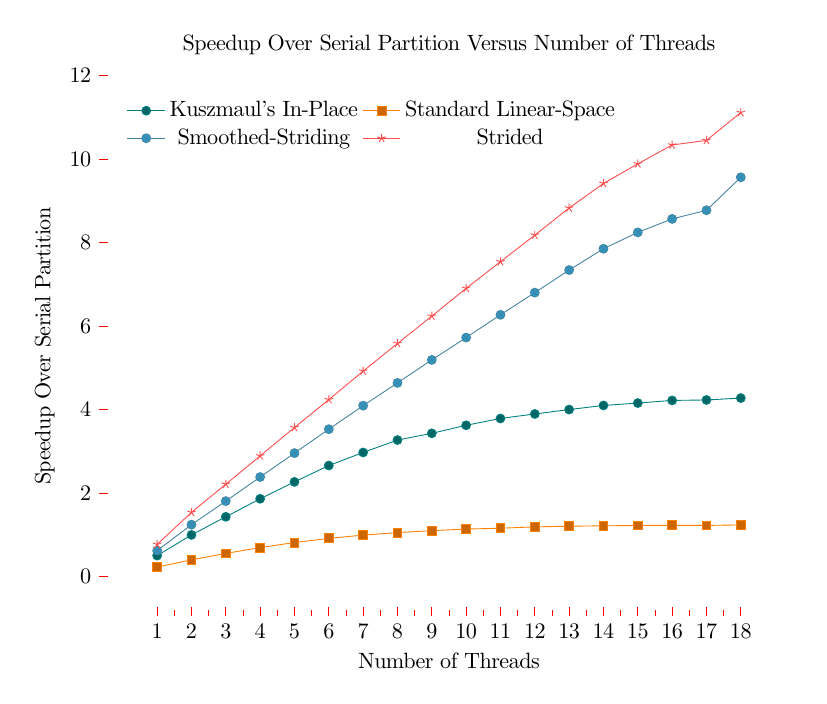
\begin{tikzpicture}[scale = .8]
\begin{axis}[
width = 5 in,
height = 4in,
title={Speedup Over Serial Partition Versus Number of Threads},
xtick pos=left,
ytick pos=left,
legend style={draw=none},
axis line style = { draw = none },
legend pos= north west,
xtick = data,
xlabel={Number of Threads},
ylabel={Speedup Over Serial Partition},
ymax = 12,
legend columns = 2,
scatter/classes=%
{a={mark=o,draw=blue}}]
%% In-Place
\addplot coordinates {( 1, 0.499048) ( 2, 0.995494) ( 3, 1.42948) ( 4, 1.86113) ( 5, 2.26614) ( 6, 2.65797) ( 7, 2.97174) ( 8, 3.26921) ( 9, 3.43004) ( 10, 3.62281) ( 11, 3.78679) ( 12, 3.89481) ( 13, 4.0002) ( 14, 4.0986) ( 15, 4.15578) ( 16, 4.2191) ( 17, 4.22999) ( 18, 4.27599) };
%% In-Place Prefix-Sum
% \addplot coordinates {( 1, 0.35092) ( 2, 0.636608) ( 3, 0.894292) ( 4, 1.11755) ( 5, 1.32674) ( 6, 1.5096) ( 7, 1.65121) ( 8, 1.77494) ( 9, 1.88432) ( 10, 1.97837) ( 11, 2.0581) ( 12, 2.11591) ( 13, 2.15699) ( 14, 2.18845) ( 15, 2.21159) ( 16, 2.21657) ( 17, 2.20736) ( 18, 2.21557) };
%% Out-of-Place
\addplot coordinates {( 1, 0.223968) ( 2, 0.398625) ( 3, 0.551717) ( 4, 0.691607) ( 5, 0.812203) ( 6, 0.912936) ( 7, 0.990429) ( 8, 1.05055) ( 9, 1.09777) ( 10, 1.13562) ( 11, 1.15517) ( 12, 1.18848) ( 13, 1.20383) ( 14, 1.21364) ( 15, 1.22103) ( 16, 1.22575) ( 17, 1.22285) ( 18, 1.23444) };
%% %% High-Span
%% \addplot coordinates {( 1, 0.796443) ( 2, 1.58021) ( 3, 2.21882) ( 4, 2.93667) ( 5, 3.32899) ( 6, 3.80217) ( 7, 4.3662) ( 8, 4.93375) ( 9, 5.09881) ( 10, 5.42822) ( 11, 5.75051) ( 12, 6.01806) ( 13, 6.37103) ( 14, 6.57999) ( 15, 6.72631) ( 16, 6.95718) ( 17, 7.06722) ( 18, 7.34442) };
%% Cache-Friendly
\addplot coordinates {( 1, 0.619888) ( 2, 1.24099) ( 3, 1.80558) ( 4, 2.38286) ( 5, 2.95654) ( 6, 3.52917) ( 7, 4.09348) ( 8, 4.63922) ( 9, 5.19034) ( 10, 5.72539) ( 11, 6.27145) ( 12, 6.80311) ( 13, 7.34442) ( 14, 7.85497) ( 15, 8.24706) ( 16, 8.57062) ( 17, 8.77723) ( 18, 9.5674) };
%% Strided
\addplot coordinates {( 1, 0.767408) ( 2, 1.5359) ( 3, 2.21084) ( 4, 2.89005) ( 5, 3.56954) ( 6, 4.2382) ( 7, 4.9214) ( 8, 5.58393) ( 9, 6.23961) ( 10, 6.90587) ( 11, 7.54451) ( 12, 8.18186) ( 13, 8.83243) ( 14, 9.4207) ( 15, 9.88984) ( 16, 10.3425) ( 17, 10.4524) ( 18, 11.1205) };
\legend{Kuszmaul's In-Place, Standard Linear-Space, Smoothed-Striding, Strided} %% Low-Space, Med-Space, High-Space, Smoothed-Striding, Strided 
\end{axis}
\end{tikzpicture}
}
\def \partitionbandwidthboundserialbaseline {3933.6}
\def \partitionbandwidthboundblocksize {64}
\def \partitionbandwidthboundnumtrials {5}
\def \partitionbandwidthboundinputsize {1073741824}
\def \partitionbandwidthboundtable {
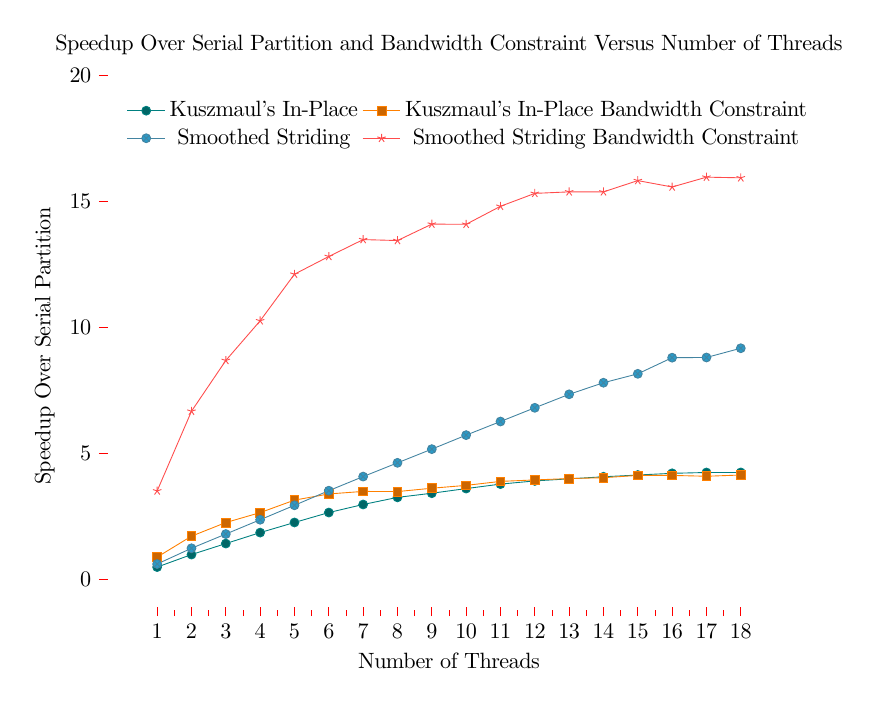
\begin{tikzpicture}[scale = .8]
\begin{axis}[
width = 5 in,
height = 4in,
title={Speedup Over Serial Partition and Bandwidth Constraint Versus Number of Threads},
xtick pos=left,
ytick pos=left,
legend style={draw=none},
axis line style = { draw = none },
legend pos= north west,
xtick = data,
xlabel={Number of Threads},
ylabel={Speedup Over Serial Partition},
ymax = 20,
legend columns = 2,
scatter/classes=%
{a={mark=o,draw=blue}}]
%% In-Place
\addplot coordinates {( 1, 0.499378) ( 2, 0.995949) ( 3, 1.4328) ( 4, 1.86816) ( 5, 2.26982) ( 6, 2.66432) ( 7, 2.98407) ( 8, 3.26602) ( 9, 3.43066) ( 10, 3.61544) ( 11, 3.79325) ( 12, 3.91949) ( 13, 4.00244) ( 14, 4.08389) ( 15, 4.15375) ( 16, 4.22151) ( 17, 4.25438) ( 18, 4.25622) };
%% Low-Space Bandwidth Bound
\addplot coordinates {(1, 0.894939)(2, 1.72634)(3, 2.26699)(4, 2.66131)(5, 3.15777)(6, 3.4024)(7, 3.50312)(8, 3.49686)(9, 3.62955)(10, 3.74294)(11, 3.90093)(12, 3.9593)(13, 4.0131)(14, 4.04714)(15, 4.13799)(16, 4.13782)(17, 4.10515)(18, 4.15355)};
%% high span
%% \addplot coordinates {( 1, 0.812828) ( 2, 1.61997) ( 3, 2.22137) ( 4, 2.95626) ( 5, 3.33582) ( 6, 3.80352) ( 7, 4.36001) ( 8, 5.10062) ( 9, 5.11521) ( 10, 5.44217) ( 11, 5.74752) ( 12, 6.07787) ( 13, 6.41278) ( 14, 6.63787) ( 15, 6.68752) ( 16, 6.79848) ( 17, 7.10549) ( 18, 7.26292) };
%% %% High-Span Bandwidth Bound
%% \addplot coordinates {(1, 1.75849)(2, 3.34185)(3, 4.35383)(4, 5.15739)(5, 5.9788)(6, 6.31621)(7, 6.76074)(8, 6.76348)(9, 6.99773)(10, 7.10173)(11, 7.39957)(12, 7.51437)(13, 7.7436)(14, 7.76191)(15, 7.89966)(16, 7.87403)(17, 7.94484)(18, 8.05483)}; %% cache friendly
\addplot coordinates {( 1, 0.62101) ( 2, 1.24639) ( 3, 1.81072) ( 4, 2.37852) ( 5, 2.95182) ( 6, 3.53233) ( 7, 4.09153) ( 8, 4.63759) ( 9, 5.18124) ( 10, 5.73746) ( 11, 6.27769) ( 12, 6.82206) ( 13, 7.35802) ( 14, 7.81717) ( 15, 8.17117) ( 16, 8.81183) ( 17, 8.81973) ( 18, 9.18636) };
%% Cache-Friendly Bandwidth Bound
\addplot coordinates {(1, 3.52223)(2, 6.68603)(3, 8.70095)(4, 10.276)(5, 12.1258)(6, 12.8292)(7, 13.4991)(8, 13.4622)(9, 14.1134)(10, 14.1066)(11, 14.8215)(12, 15.3338)(13, 15.3938)(14, 15.3942)(15, 15.8412)(16, 15.5877)(17, 15.9778)(18, 15.9519)};
\legend{Kuszmaul's In-Place, Kuszmaul's In-Place Bandwidth Constraint, Smoothed Striding, Smoothed Striding Bandwidth Constraint}
\end{axis}
\end{tikzpicture}
}

\def \CILKsortblocksize {64}
\def \CILKsortnumtrials {5}
\def \CILKsortmaxinputsize {1073741824}
\def \CILKsorttable {
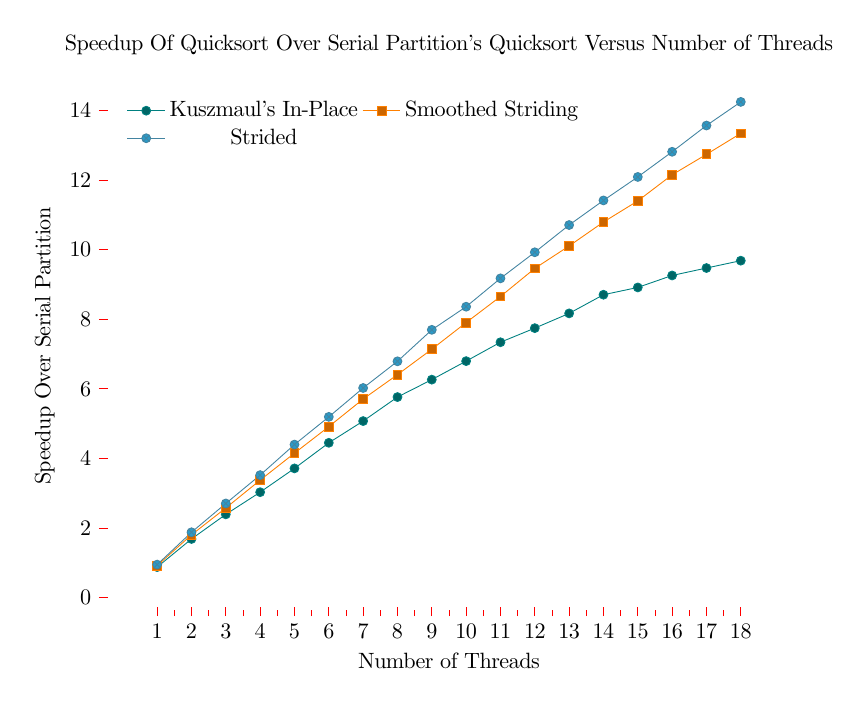
\begin{tikzpicture}[scale = .8]
\begin{axis}[
width = 5 in,
height = 4in,
title={Speedup Of Quicksort Over Serial Partition's Quicksort Versus Number of Threads},
xtick pos=left,
ytick pos=left,
legend style={draw=none},
axis line style = { draw = none },
legend pos= north west,
xtick = data,
xlabel={Number of Threads},
ylabel={Speedup Over Serial Partition},
ymax = 15,
legend columns = 2,
scatter/classes=%
{a={mark=o,draw=blue}}]
%% %% Low Space with log size 24
%% \addplot coordinates {( 1, 0.863202) ( 2, 1.63232) ( 3, 2.29705) ( 4, 2.96413) ( 5, 3.59298) ( 6, 4.1696) ( 7, 4.71085) ( 8, 5.2279) ( 9, 5.8474) ( 10, 6.4043) ( 11, 6.55736) ( 12, 7.21241) ( 13, 7.57064) ( 14, 7.99417) ( 15, 8.4679) ( 16, 8.93099) ( 17, 9.04881) ( 18, 9.60644) %% High-Span with log size 24
%% \addplot coordinates {( 1, 0.960106) ( 2, 1.88538) ( 3, 2.72075) ( 4, 3.47467) ( 5, 4.2576) ( 6, 5.08451) ( 7, 5.93339) ( 8, 6.47686) ( 9, 7.1822) ( 10, 7.57901) ( 11, 8.44704) ( 12, 8.64943) ( 13, 9.16979) ( 14, 9.04881) ( 15, 10.1464) ( 16, 9.61992) ( 17, 10.5199) ( 18, 9.38304) %% Cache Friendly with log size 24
%% \addplot coordinates {( 1, 0.900013) ( 2, 1.74752) ( 3, 2.46372) ( 4, 3.23233) ( 5, 3.90159) ( 6, 4.62508) ( 7, 5.46099) ( 8, 6.15157) ( 9, 6.85215) ( 10, 7.53736) ( 11, 8.11716) ( 12, 8.74872) ( 13, 9.70156) ( 14, 9.04881) ( 15, 11.0273) ( 16, 10.87) ( 17, 12.1829) ( 18, 12.2482) %% Strided with log size 24
%% \addplot coordinates {( 1, 0.95079) ( 2, 1.82955) ( 3, 2.63808) ( 4, 3.45716) ( 5, 4.20798) ( 6, 4.99199) ( 7, 5.78819) ( 8, 6.56364) ( 9, 7.37527) ( 10, 8.03162) ( 11, 8.89624) ( 12, 9.61992) ( 13, 9.7153) ( 14, 11.1167) ( 15, 10.9394) ( 16, 11.4891) ( 17, 13.1651) ( 18, 13.9695) };
%% %% Low Space with log size 26
%% \addplot coordinates {( 1, 0.861043) ( 2, 1.63325) ( 3, 2.3004) ( 4, 2.98343) ( 5, 3.63316) ( 6, 4.19898) ( 7, 4.82886) ( 8, 5.34581) ( 9, 5.89992) ( 10, 6.44372) ( 11, 6.94206) ( 12, 7.4672) ( 13, 7.60676) ( 14, 8.0564) ( 15, 8.64475) ( 16, 8.82709) ( 17, 8.76202) ( 18, 8.96831) %% High-Span with log size 26
%% \addplot coordinates {( 1, 0.955523) ( 2, 1.86586) ( 3, 2.6845) ( 4, 3.49224) ( 5, 4.27081) ( 6, 5.0929) ( 7, 5.83274) ( 8, 6.53586) ( 9, 7.29308) ( 10, 7.90003) ( 11, 8.63721) ( 12, 8.97915) ( 13, 9.7769) ( 14, 10.1893) ( 15, 10.5812) ( 16, 10.7887) ( 17, 10.7613) ( 18, 10.3418) %% Cache Friendly with log size 26
%% \addplot coordinates {( 1, 0.914609) ( 2, 1.73339) ( 3, 2.49178) ( 4, 3.22151) ( 5, 4.02384) ( 6, 4.70946) ( 7, 5.57239) ( 8, 6.13884) ( 9, 6.93881) ( 10, 7.59315) ( 11, 8.23047) ( 12, 8.91717) ( 13, 9.42939) ( 14, 10.1302) ( 15, 10.6801) ( 16, 10.8359) ( 17, 11.3883) ( 18, 11.3189) %% Strided with log size 26
%% \addplot coordinates {( 1, 0.946785) ( 2, 1.82922) ( 3, 2.64766) ( 4, 3.4262) ( 5, 4.2788) ( 6, 5.08245) ( 7, 5.95192) ( 8, 6.67986) ( 9, 7.44475) ( 10, 8.25563) ( 11, 8.94132) ( 12, 9.74164) ( 13, 10.4362) ( 14, 11.3621) ( 15, 11.4851) ( 16, 12.2071) ( 17, 12.6542) ( 18, 13.4993) };
%% %% Low Space with log size 28
%% \addplot coordinates {( 1, 0.862267) ( 2, 1.63941) ( 3, 2.34664) ( 4, 2.96157) ( 5, 3.64611) ( 6, 4.31258) ( 7, 4.88345) ( 8, 5.43042) ( 9, 5.87762) ( 10, 6.44029) ( 11, 7.00878) ( 12, 7.30452) ( 13, 7.83539) ( 14, 8.12956) ( 15, 8.50856) ( 16, 8.76302) ( 17, 8.98741) ( 18, 9.33821) %% High-Span with log size 28
%% \addplot coordinates {( 1, 0.939362) ( 2, 1.84744) ( 3, 2.6917) ( 4, 3.45716) ( 5, 4.29244) ( 6, 5.08279) ( 7, 5.79208) ( 8, 6.6353) ( 9, 7.2093) ( 10, 8.01682) ( 11, 8.74742) ( 12, 9.17326) ( 13, 9.7479) ( 14, 10.2979) ( 15, 11.0745) ( 16, 11.4344) ( 17, 11.4888) ( 18, 12.34) %% Cache Friendly with log size 28
%% \addplot coordinates {( 1, 0.908881) ( 2, 1.75263) ( 3, 2.51771) ( 4, 3.28228) ( 5, 4.01042) ( 6, 4.74982) ( 7, 5.54834) ( 8, 6.2393) ( 9, 6.98884) ( 10, 7.70125) ( 11, 8.41219) ( 12, 9.06778) ( 13, 9.67555) ( 14, 10.3505) ( 15, 11.0125) ( 16, 11.4744) ( 17, 12.1533) ( 18, 12.4095) %% Strided with log size 28
%% \addplot coordinates {( 1, 0.942529) ( 2, 1.82563) ( 3, 2.6044) ( 4, 3.46053) ( 5, 4.25683) ( 6, 5.12315) ( 7, 5.88602) ( 8, 6.70811) ( 9, 7.43113) ( 10, 8.17952) ( 11, 8.96974) ( 12, 9.68435) ( 13, 10.4214) ( 14, 10.9587) ( 15, 11.71) ( 16, 12.2949) ( 17, 12.9046) ( 18, 13.3107) };
%% Low Space with log size 30
\addplot coordinates {( 1, 0.87864) ( 2, 1.68661) ( 3, 2.39404) ( 4, 3.03172) ( 5, 3.71549) ( 6, 4.45118) ( 7, 5.07595) ( 8, 5.76618) ( 9, 6.26716) ( 10, 6.79929) ( 11, 7.34223) ( 12, 7.74736) ( 13, 8.17148) ( 14, 8.70784) ( 15, 8.91736) ( 16, 9.26139) ( 17, 9.47532) ( 18, 9.68665)}; %% High-Span with log size 30
%% \addplot coordinates {( 1, 0.96225) ( 2, 1.879) ( 3, 2.71741) ( 4, 3.56118) ( 5, 4.44821) ( 6, 5.29223) ( 7, 5.97895) ( 8, 6.76091) ( 9, 7.59373) ( 10, 8.37912) ( 11, 9.01587) ( 12, 9.58729) ( 13, 10.1906) ( 14, 10.881) ( 15, 11.4166) ( 16, 12.026) ( 17, 12.3279) ( 18, 12.6408)}; %% Cache Friendly with log size 30
\addplot coordinates {( 1, 0.921182) ( 2, 1.80562) ( 3, 2.57745) ( 4, 3.37831) ( 5, 4.15358) ( 6, 4.91613) ( 7, 5.7093) ( 8, 6.41041) ( 9, 7.14098) ( 10, 7.907) ( 11, 8.6573) ( 12, 9.46479) ( 13, 10.1098) ( 14, 10.7975) ( 15, 11.4046) ( 16, 12.1549) ( 17, 12.7427) ( 18, 13.346)}; %% Strided with log size 30
\addplot coordinates {( 1, 0.949951) ( 2, 1.87888) ( 3, 2.70758) ( 4, 3.52248) ( 5, 4.40049) ( 6, 5.19675) ( 7, 6.02708) ( 8, 6.79362) ( 9, 7.69896) ( 10, 8.36354) ( 11, 9.17828) ( 12, 9.92823) ( 13, 10.7114) ( 14, 11.4187) ( 15, 12.0935) ( 16, 12.8171) ( 17, 13.5719) ( 18, 14.2507) };
\legend{Kuszmaul's In-Place, Smoothed Striding, Strided}
\end{axis}
\end{tikzpicture}
}

%% Bandwith results without numactl:
%% \def \partitionbandwidthboundserialbaseline {3832}
%% \def \partitionbandwidthboundblocksize {64}
%% \def \partitionbandwidthboundnumtrials {5}
%% \def \partitionbandwidthboundinputsize {1073741824}
%% \def \partitionbandwidthboundtable {
%% \begin{tikzpicture}[scale = .8]
%% \begin{axis}[
%% width = 5 in,
%% height = 4in,
%% title={Speedup Versus Number of Threads},
%% xtick pos=left,
%% ytick pos=left,
%% legend style={draw=none},
%% axis line style = { draw = none },
%% legend pos= north west,
%% xtick = data,
%% xlabel={Number of Threads},
%% ylabel={Speedup Over Serial Partition},
%% ymax = 4,
%% legend columns = 2,
%% scatter/classes=%
%% {a={mark=o,draw=blue}}]
%% %% In-Place
%% \addplot coordinates {( 1, 0.504928) ( 2, 0.744917) ( 3, 1.27793) ( 4, 1.62967) ( 5, 1.91677) ( 6, 2.3244) ( 7, 2.47865) ( 8, 2.58186) ( 9, 2.68573) ( 10, 2.78448) ( 11, 2.7756) ( 12, 2.85077) ( 13, 2.86826) ( 14, 2.91407) ( 15, 2.90479) ( 16, 2.94769) ( 17, 2.95497) ( 18, 2.94588) };
%% %% Low-Space Bandwidth Bound
%% \addplot coordinates {(1, 1.05385)(2, 1.63936)(3, 1.81183)(4, 2.05614)(5, 2.39067)(6, 2.5237)(7, 2.40513)(8, 2.55015)(9, 2.58884)(10, 2.57444)(11, 2.69167)(12, 2.66946)(13, 2.64859)(14, 2.68175)(15, 2.66023)(16, 2.69318)(17, 2.68783)(18, 2.72913)};
%% %% high span
%% \addplot coordinates {( 1, 0.816814) ( 2, 1.47691) ( 3, 1.98529) ( 4, 2.63875) ( 5, 3.01305) ( 6, 3.40441) ( 7, 3.68887) ( 8, 3.97345) ( 9, 4.14181) ( 10, 4.27297) ( 11, 4.46724) ( 12, 4.45271) ( 13, 4.45271) ( 14, 4.62355) ( 15, 4.60024) ( 16, 4.70184) ( 17, 4.55431) ( 18, 4.71225) };
%% %% High-Span Bandwidth Bound
%% \addplot coordinates {(1, 2.03744)(2, 3.14521)(3, 3.47353)(4, 3.91661)(5, 4.536)(6, 4.70395)(7, 4.47075)(8, 4.76355)(9, 4.86065)(10, 4.68934)(11, 4.86418)(12, 4.98468)(13, 4.9239)(14, 4.99117)(15, 4.94174)(16, 4.98761)(17, 4.96382)(18, 5.00564)%% cache friendly
%% \addplot coordinates {( 1, 0.621291) ( 2, 1.06581) ( 3, 1.76541) ( 4, 2.28204) ( 5, 2.8838) ( 6, 3.49253) ( 7, 4.04561) ( 8, 4.56843) ( 9, 4.97921) ( 10, 5.6089) ( 11, 5.8791) ( 12, 6.26963) ( 13, 6.8331) ( 14, 6.87971) ( 15, 7.15459) ( 16, 7.38343) ( 17, 8.25151) ( 18, 8.35587) };
%% %% Cache-Friendly Bandwidth Bound
%% \addplot coordinates {(1, 4.06363)(2, 6.29023)(3, 6.9299)(4, 7.88794)(5, 9.08502)(6, 9.329)(7, 9.45987)(8, 9.53406)(9, 9.91163)(10, 9.90729)(11, 9.70433)(12, 10.1146)(13, 9.9126)(14, 9.85886)(15, 9.86993)(16, 10.0183)(17, 10.0765)(18, 9.99261)};
%% \legend{Low-Space, Low-Space Bandwidth Constraint, Two-Layer, Two-Layer Bandwidth Constraint}
%% \end{axis}
%% \end{tikzpicture}
%% }

\def \serialnumtrials {5}
\def \serialblocksize {64}
\def \serialtable {
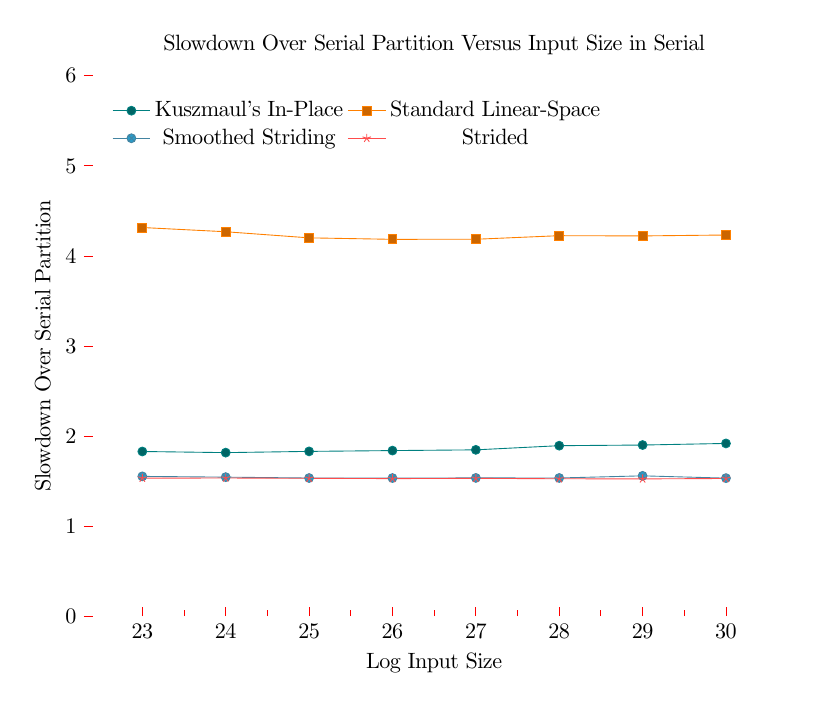
\begin{tikzpicture}[scale = .8]
\begin{axis}[
width = 5 in,
height = 4in,
title={Slowdown Over Serial Partition Versus Input Size in Serial},
xtick pos=left,
ytick pos=left,
ymax = 6,
ymin = 0,
legend style={draw=none},
axis line style = { draw = none },
legend pos= north west,
xtick = data,
xlabel={Log Input Size},
ylabel={Slowdown Over Serial Partition},
legend columns = 2,
scatter/classes=%
{a={mark=o,draw=blue}}]
%% Serial Baseline
%% baselines in ms: \addplot coordinates {( 23, 30.4 ) ( 24, 61 ) ( 25, 122.4 ) ( 26, 244.8 ) ( 27, 489.6 ) ( 28, 979.6 ) ( 29, 1963.4 ) ( 30, 3922.6 ) };
%% In-Place
\addplot coordinates {( 23, 1.82895) ( 24, 1.81639) ( 25, 1.83007) ( 26, 1.83905) ( 27, 1.84722) ( 28, 1.89343) ( 29, 1.90068) ( 30, 1.91837) };
%% In-Place Prefix-Sum
% \addplot coordinates {( 23, 2.75658) ( 24, 2.71803) ( 25, 2.68137) ( 26, 2.67157) ( 27, 2.67443) ( 28, 2.70131) ( 29, 2.70551) ( 30, 2.71713) };
%% Out-of-Place
\addplot coordinates {( 23, 4.31579) ( 24, 4.26885) ( 25, 4.20098) ( 26, 4.18464) ( 27, 4.18546) ( 28, 4.22519) ( 29, 4.22257) ( 30, 4.23265) };
%% %% High-Span
%% \addplot coordinates {( 23, 1.23684) ( 24, 1.23934) ( 25, 1.24346) ( 26, 1.24428) ( 27, 1.24632) ( 28, 1.24602) ( 29, 1.24417) ( 30, 1.2456) };
%% Cache-Friendly
\addplot coordinates {( 23, 1.55263) ( 24, 1.54426) ( 25, 1.53431) ( 26, 1.53431) ( 27, 1.53554) ( 28, 1.53491) ( 29, 1.55852) ( 30, 1.53317) };
%% Strided
\addplot coordinates {( 23, 1.53289) ( 24, 1.53443) ( 25, 1.53105) ( 26, 1.52778) ( 27, 1.53064) ( 28, 1.52613) ( 29, 1.5246) ( 30, 1.52919) };
\legend{Kuszmaul's In-Place, Standard Linear-Space, Smoothed Striding, Strided} % Low-Space, Med-Space, High-Space, Smoothed Striding, Strided
\end{axis}
\end{tikzpicture}
}
%% \def \serialnumtrials {5}
%% \def \serialblocksize {64}
%% \def \serialtable {
%% \begin{tikzpicture}[scale = .8]
%% \begin{axis}[
%% width = 5 in,
%% height = 4in,
%% title={Slowdown Versus Input Size in Serial},
%% xtick pos=left,
%% ytick pos=left,
%% ymax = 5,
%% ymin = 0,
%% legend style={draw=none},
%% axis line style = { draw = none },
%% legend pos= north west,
%% xtick = data,
%% xlabel={Log Input Size},
%% ylabel={Slowdown Over Serial Partition},
%% legend columns = 2,
%% scatter/classes=%
%% {a={mark=o,draw=blue}}]
%% %% Serial Baseline
%% %% baselines in ms: \addplot coordinates {( 23, 30.4 ) ( 24, 61 ) ( 25, 122.4 ) ( 26, 244.8 ) ( 27, 489.6 ) ( 28, 979.6 ) ( 29, 1963.4 ) ( 30, 3922.6 ) };
%% %% In-Place
%% \addplot coordinates {( 23, 1.82895) ( 24, 1.81639) ( 25, 1.83007) ( 26, 1.83905) ( 27, 1.84722) ( 28, 1.89343) ( 29, 1.90068) ( 30, 1.91837) };
%% %% In-Place Prefix-Sum
%% \addplot coordinates {( 23, 2.75658) ( 24, 2.71803) ( 25, 2.68137) ( 26, 2.67157) ( 27, 2.67443) ( 28, 2.70131) ( 29, 2.70551) ( 30, 2.71713) };
%% %% Out-of-Place
%% \addplot coordinates {( 23, 4.31579) ( 24, 4.26885) ( 25, 4.20098) ( 26, 4.18464) ( 27, 4.18546) ( 28, 4.22519) ( 29, 4.22257) ( 30, 4.23265) };
%% %% High-Span
%% \addplot coordinates {( 23, 1.23684) ( 24, 1.23934) ( 25, 1.24346) ( 26, 1.24428) ( 27, 1.24632) ( 28, 1.24602) ( 29, 1.24417) ( 30, 1.2456) };
%% %% Cache-Friendly
%% \addplot coordinates {( 23, 1.55263) ( 24, 1.54426) ( 25, 1.53431) ( 26, 1.53431) ( 27, 1.53554) ( 28, 1.53491) ( 29, 1.55852) ( 30, 1.53317) };
%% %% Strided
%% \addplot coordinates {( 23, 1.53289) ( 24, 1.53443) ( 25, 1.53105) ( 26, 1.52778) ( 27, 1.53064) ( 28, 1.52613) ( 29, 1.5246) ( 30, 1.52919) };
%% \legend{Low-Space, Med-Space, High-Space, Two-Layer, Cache-Friendly, Strided}
%% \end{axis}
%% \end{tikzpicture}
%% }
%% \def \serialnumtrials {1}
%% \def \serialblocksize {64}
%% \def \serialtable {
%% \begin{tikzpicture}[scale = .8]
%% \begin{axis}[
%% title={Slowdown Versus Input Size in Serial},
%% width = 5in, %%!!!!
%% height = 4in,
%% xtick pos=left,
%% ytick pos=left,
%% ymax = 5, %% !!!
%% ymin = 0,
%% legend style={draw=none},
%% axis line style = { draw = none },
%% legend pos= north west,
%% xtick = data,
%% xlabel={Log Input Size},
%% ylabel={Slowdown Over Serial Partition},
%% legend columns = 2,
%% scatter/classes=%
%% {a={mark=o,draw=blue}}]
%% %% Serial Baseline%% baselines in ms: \addplot coordinates {( 23, 30.4 ) ( 24, 60.8 ) ( 25, 121.4 ) ( 26, 243.8 ) ( 27, 487.4 ) ( 28, 975.8 ) ( 29, 1952.2 ) ( 30, 3902 ) };
%% %% In-Place
%% \addplot coordinates {( 23, 1.79605) ( 24, 1.82237) ( 25, 1.84185) ( 26, 1.84249) ( 27, 1.87033) ( 28, 1.90838) ( 29, 1.90687) ( 30, 1.91579) };
%% %% In-Place Prefix-Sum
%% \addplot coordinates {( 23, 2.58553) ( 24, 2.57237) ( 25, 2.57661) ( 26, 2.56932) ( 27, 2.56422) ( 28, 2.59459) ( 29, 2.60834) ( 30, 2.61107) };
%% %% Out-of-Place
%% \addplot coordinates {( 23, 3.98684) ( 24, 3.96711) ( 25, 3.96705) ( 26, 3.96308) ( 27, 3.98195) ( 28, 4.01537) ( 29, 4.03401) ( 30, 4.06079) };
%% %% High-Span
%% \addplot coordinates {( 23, 1.21053) ( 24, 1.23355) ( 25, 1.23558) ( 26, 1.23298) ( 27, 1.23677) ( 28, 1.24124) ( 29, 1.24096) ( 30, 1.23931) };
%% \legend{Low-Space, Med-Space, High-Space, Two-Layer} %% Two-layer instead of high-span everywhere
%% \end{axis}
%% \end{tikzpicture}
%% }
%% %% Speedup on 18 threads in table of size 268435456
%% \def \serialsortspeedup {0.780189}


\newcommand{\dec}{\operatorname{dec}}
\newcommand{\poly}{\operatorname{poly}}
\newcommand{\polylog}{\operatorname{polylog}}
\newcommand{\github}{\url{github.com/awestover/Parallel-Partition}}
\newcommand{\defn}[1]{{\textit{\textbf{\boldmath #1}}} }
\renewcommand{\paragraph}[1]{\vspace{0.09in}\noindent{\bf \boldmath #1.}} 
\usepackage{amsmath}
\def\E{\operatorname{\mathbb{E}}}
\usepackage{amssymb}
\usepackage{amsthm}
\usepackage{todonotes}

\newtheorem{thm}{Theorem}[section]
\newtheorem{lem}[thm]{Lemma}
\newtheorem{prop}[thm]{Proposition}
\newtheorem{clm}[thm]{Claim}
\newtheorem{cor}[thm]{Corollary}
\newtheorem{conj}[thm]{Conjecture}
\theoremstyle{remark}
\newtheorem{rem}[thm]{Remark}
\newtheorem{ex}[thm]{Example}

\newtheorem{theorem}{Theorem}[section]
\newtheorem{definition}[thm]{Definition}
\newtheorem{lemma}[thm]{Lemma}
\newtheorem{proposition}[thm]{Proposition}
\newtheorem{claim}[thm]{Claim}
\newtheorem{corollary}[thm]{Corollary}
\newtheorem{conjecture}[thm]{Conjecture}
\theoremstyle{remark}
\newtheorem{remark}[thm]{Remark}
\newtheorem{example}[thm]{Example}
\newtheorem{observation}[thm]{Observation}

\usepackage{hyperref}
\usepackage{cite}
\usepackage{natbib}


\begin{document}
\title{Cache-Efficient Parallel-Partition Algorithms \\using Exclusive-Read-and-Write Memory}

\author{William Kuszmaul}
% \affiliation{ \institution{Massachusetts Institute of Technology} }
% \email{kuszmaul@mit.edu}


\author{Alek Westover}
% \authornote{Supported by MIT PRIMES.}
% \email{alek.westover@gmail.com}

% The default list of authors is too long for headers.
% \renewcommand{\shortauthors}{Alek Westover}

\begin{titlepage}
    \begin{center}
        \vspace*{1cm}
 
        \Huge
        \textbf{Cache-Efficient Parallel-Partition Algorithms using Exclusive-Read-and-Write Memory}
 
        \vspace{0.5cm}
        \LARGE
				An In-Place Algorithm With Provably Optimal Cache Behavior
 
        \vspace{1.5cm}
				\vfill
 
        \textbf{Alek Westover}

        \vspace{1.5cm}
				Belmont High School

				Massachusetts, USA

        \vspace{1.5cm}
				Mentor: William Kuszmaul (MIT)
 
        \vspace{0.8cm}
				MIT PRIMES Computer Science Research Program
 
 
        \Large
 
    \end{center}
\end{titlepage}


\maketitle
\begin{abstract} The parallel-partition problem, which is essential to Parallel
	Quicksort and appears in many other algorithms, is given an array $A$ of
	length $n$, and must partition the array based on some pivot property. The
	standard solution to the parallel-partition problem is out-of-place. Having
	an in-place algorithm is desirable because it makes the algorithm faster in
	practice and because sorting problems are often memory intensive so extra
	space may be undesirable or high cost. Kuszmaul developed an in-place
	algorithm for the parallel-partition problem, but the algorithm performs
	multiple passes over the array and thus its performance is bottlenecked by
	memory-bandwidth. The Blocked Strided Algorithm of Francis, Pannan, Frias, and
	Petit is in-place and under certain conditions performs little more than a
	single pass over the array. Because of this, for certain inputs the Blocked
	Strided Algorithm incurs very few cache misses and thus performs well.
	However in general this algorithm has no theoretical guarantees on span and
	cache-behavior.

	We present an in-place EREW algorithm with polylogarithmic span and provably
	optimal cache behavior, up to small-order factors.  The resulting algorithm
	achieves near-ideal scaling in practice by avoiding the memory-bandwidth
	bottleneck. The algorithm's performance is comparable to that of the Blocked
	Strided Algorithm, the previous state-of-the art for parallel EREW sorting
	algorithms.

% This means that they can be implemented using only parallel for loops, and do
	% not require the use of any concurrency mechanisms such as locks or atomic
	% variables. Despite the parallel-partition problem being heavily studied, no
	% algorithms have achieved these theoretical guarantees before.

\end{abstract}




 

\section{Introduction}

A \defn{parallel partition} operation rearranges the elements in an
array so that the elements satisfying a particular \defn{pivot
  property} appear first. In addition to playing a central role in
parallel quicksort, the parallel partition operation is used as a
primitive throughout parallel algorithms.\footnote{In several
  well-known textbooks and surveys on parallel algorithms
  \cite{AcarBl16,Blelloch96}, for example, parallel partitions are
  implicitly used extensively to perform what are referred to as
  \emph{filter} operations.}

A parallel algorithm's performance can be measured by its \defn{work}, the time
needed to execute in serial, and its \defn{span}, the time needed to execute
on infinitely many processors. There is a well-known algorithm for
parallel partition on arrays of size $n$ with work $O(n)$ and span
$O(\log n)$ \cite{Blelloch96,AcarBl16}. Moreover, the algorithm uses
only exclusive read/write shared memory variables (i.e., it is an
\defn{EREW} algorithm). This eliminates the need for concurrency
mechanisms such as locks and atomic variables, and ensures good
behavior even if the time to access a location is a function of the
number of threads trying to access it (or its cache line)
concurrently. EREW algorithms also have the advantage that their
behavior is internally deterministic, meaning that
the behavior of the algorithm will not differ from run to run, which
makes test coverage, debugging, and reasoning about performance
substantially easier \cite{BlellochFi12}.

This parallel-partition algorithm suffers from using a large amount of
auxiliary memory, however. Whereas the serial algorithm is typically
implemented in place, the parallel algorithm relies on the use of two
auxiliary arrays of size $n$. To the best of our knowledge, the only
known linear-work and $\operatorname{polylog}(n)$-span algorithms for
parallel partition that are in-place require the use of atomic
operations (e.g, fetch-and-add)
\cite{HeidelbergerNo90,AxtmannWi17,TsigasZh03}.

An algorithm's memory efficiency can be critical on large inputs. The
memory consumption of an algorithm determines the largest problem size
that can be executed in memory. Many external memory algorithms (i.e.,
algorithms for problems too large to fit in memory) perform large
subproblems in memory; the size of these subproblems is again
bottlenecked by the algorithm's memory-overhead \cite{Vitter08}. In
multi-user systems, processes with larger memory-footprints can hog
the cache and the memory bandwidth, slowing down other processes.

For sorting algorithms, in particular, special attention to memory
efficiency is often given. This is because (a) a user calling the sort
function may already be using almost all of the memory in the system;
and (b) sorting algorithms, and especially parallel sorting
algorithms, are often bottlenecked by memory bandwidth. The latter
property, in particular, means that any parallel sorting algorithm
that wishes to achieve state-of-the art performance on a large
multi-processor machine must be (at least close to) in place.

Currently the only practical in-place parallel sorting algorithms
either rely heavily on atomic operations or other concurrency
mechanisms \cite{HeidelbergerNo90, AxtmannWi17, TsigasZh03}, or eschew
theoretical guarantees \cite{FrancisPa92}. Parallel merge sort
\cite{Hagerup89} was made in-place by Katajainen \cite{Katajainen93},
but has proven too sophisticated for practical applications. Bitonic
sort \cite{BlellochLe98} is naturally in-place, and can be practical
in certain applications on super computers, but suffers in general
from requiring work $\Theta(n \log^2 n)$ rather than $O(n \log
n)$. Parallel quicksort, on the other hand, despite the many efforts
to optimize it \cite{HeidelbergerNo90, AxtmannWi17, TsigasZh03,
  FrancisPa92, Frias08}, has eluded any in-place EREW (or CREW)
algorithms due to its reliance on parallel partition.\footnote{In a \defn{CREW}
algorithm, reads may be concurrent, but writes may not. CREW stands for
\emph{concurrent-read exclusive-write}.}

\paragraph{Results}
We consider the problem of designing a theoretically efficient
parallel-partition algorithm that also performs well in practice. All
of the algorithms considered in this paper use only exclusive
read/write shared variables, and can be implemented using
parallel-for-loops without any additional concurrency considerations.

We give a simple parallel-partition algorithm that simultaneously
achieves good theoretical guarantees and near state-of-the-art
empirical performance. In addition to incurring linear work and
polylogarithmic span, the algorithm exhibits provably optimal cache
behavior up to low-order terms. In particular, if the input consists
of $m$ cache lines, then the algorithm incurs at most $m(1 + o(1))$ cache misses,
with high probability in $m$.

Concurrent work to ours has also developed a suite of techniques for
transforming the standard linear-space parallel partition algorithm
into an in-place algorithm \cite{Kuszmaul19}. The new algorithm, which
we call Kuszmaul's algorithm \cite{Kuszmaul19}, is able to achieve a
speedup over the linear-space algorithm due to its increased cache
efficiency. Kuszmaul's algorithm does not exhibit optimal cache
behavior, however, and as we show in our experimental evaluation, the
algorithm remains bottlenecked by memory throughput. In contrast, the
cache-optimality of our algorithm eliminates the memory-throughput
bottleneck, allowing for nearly perfect scaling on many processors.

The memory-bandwidth bottleneck has led past researchers
\cite{FrancisPa92, Frias08} to introduce the so-called \defn{Strided
  Algorithm}, which has near optimal cache behavior in practice, but
which exhibits theoretical guarantees only on certain random input
arrays. The Strided Algorithm demonstrates the empirical importance of
cache-behavior in the parallel-partition problem.

Our algorithm, which we call the \defn{Smoothed Striding Algorithm} is
designed to have similar empirical performance to the Strided
Algorithm, while achieving both theoretical guarantees on work/span
and on cache-optimality. This is achieved by randomly perturbing the
internal structure of the Strided Algorithm, and adding a recursion
step that was previously not possible. The Smoothed Striding Algorithm
is in-place, has polylogarithmic span, and exhibits provably optimal
cache behavior up to small-order factors. In practice, the Smoothed
Striding Algorithm performs within 15\% of the Strided Algorithm on a
large number of threads.




%% We will highlight past work demonstrating that parallel partition can be
%% implemented in place. However, this in-place implementation remains
%% bottlenecked by memory bandwidth, due to the fact that multiple passes over the
%% input array are required. 

%% The memory-bandwidth bottleneck has led past researchers \cite{FrancisPa92,
%% Frias08} to introduce the so-called \defn{Strided Algorithm}, which has near
%% optimal cache behavior in practice, but which exhibits theoretical guarantees
%% only on certain inputs such as random input arrays.

%% Our main result is an algorithm that we call the \defn{Smoothed Striding
%% Algorithm}. By randomly perturbing the internal structure of the Strided
%% Algorithm, and adding a recursion step that was previously not possible, we
%% arrive at a new algorithm with provably good span and cache behavior. The
%% Smoothed Striding Algorithm is in-place, has polylogarithmic span, and exhibits
%% provably optimal cache behavior up to small-order factors. In practice, the
%% Smoothed Striding Algorithm performs within 15\% of the Strided Algorithm on a
%% large number of threads.


\section{Preliminaries}\label{secprelim}

We begin by describing the the parallelism and memory model used in the paper,
and by presenting background on parallel partition.

\paragraph{Workflow Model} We consider a simple language-based model of
parallelism in which algorithms achieve parallelism through the use of
\defn{parallel-for-loops} (see, e.g.,
\cite{Blelloch96,AcarBl16,CLRS}).  Function calls within
parallel-for-loops then allow for more complicated parallel structures
(e.g., recursion). Our algorithms can also be implemented in the less
restrictive PRAM model \cite{Blelloch96, AcarBl16}.

Formally, a parallel-for-loop is given a range $R \in \mathbb{N}$, a constant
number of arguments $\arg_1, \arg_2, \ldots, \arg_c$, and a body of code. For
each $i \in \{1, \ldots, R\}$, the loop launches a thread that is given
loop-counter $i$ and local copies of the arguments $\arg_1, \arg_2, \ldots,
\arg_c$. The threads are then taken up by processors and the iterations of the
loop are performed in parallel. Only after every iteration of the loop is
complete can control flow continue past the loop.

A parallel algorithm may be run on an arbitrary number $p$ of
processors. The algorithm itself is oblivious to $p$, however, leaving
the assignment of threads to processors up to a scheduler.

The \defn{work} $T_1$ of an algorithm is the time that the algorithm
would require to execute on a single processor. The \defn{span}
$T_\infty$ of an algorithm is the time to execute on infinitely many
processors. The scheduler is assumed to contribute no overhead to the
span. In particular, if each iteration of a
parallel-for-loop has span $s$, then the full parallel loop has span
$s + O(1)$ \cite{Blelloch96,AcarBl16}.

The work $T_1$ and span $T_\infty$ can be used to quantify the time $T_p$
that an algorithm requires to execute on $p$ processors using a greedy
online scheduler. If the scheduler is assumed to contribute no
overhead, then Brent's Theorem \cite{Brent74} states that for any
$p$,
$$T_1 / p \le T_p \le T_1 / p + T_\infty.$$

The work-stealing algorithms used in the Cilk extension of C/C++ realize
the guarantee offered by Brent's Theorem within a constant factor
\cite{BlumofeJo96,BlumofeLe99}, with the added caveat that parallel-for-loops
typically induce an additional additive overhead of $O(\log R)$. 

\paragraph{Memory Model} Memory is \defn{exclusive-read} and \defn{exclusive-write}. That is, no two threads are ever permitted to attempt to read or write to the same variable concurrently. 
The exclusive-read exclusive-write memory model is sometime referred
to as the \defn{EREW model} (see, e.g., \cite{Hagerup89}).

Note that threads are not in lockstep (i.e., they may progress at arbitrary different speeds), and thus the EREW model requires algorithms to be data-race free in order to avoid the possibility of non-exclusive data accesses.

In an \defn{in-place} algorithm, each thread is given $O(\polylog(n))$
memory upon creation that is deallocated when the thread dies. This
memory can be shared with the thread's children. However, the depth of
the parent-child tree is not permitted to exceed $O(\polylog(n))$.

Whereas the EREW memory model prohibits concurrent accesses to memory, on the
other side of the spectrum are CRCW (concurrent-read-concurrent-write) models,
which allow for both reads and writes to be performed concurrently (and in some
variants even allow for atomic operations)
\cite{Blelloch96,AcarBl16,MatiasVi95}. One approach to designing efficient EREW
algorithms is to simulate efficient CRCW algorithms in the EREW model
\cite{MatiasVi95}. The known simulation techniques require substantial space
overhead, however, preventing the design of in-place algorithms
\cite{MatiasVi95}.\footnote{The known simulation techniques also increase the
total work in the original algorithm, although this can be acceptable if only a
small number of atomic operations need to be simulated.}

%% HERE: Is where we can talk about the more powerful alternative to EREW, and there relationship, and why we can't just simulate CRCW (or, more importantly, ERCW). Make it clear that the Exclusive Read part is not actually very important -- it's the exclusive write part that's hard.

%% \footnote{The
  %% algorithm in this paper satisfies a slightly stronger property that
  %% the total memory being used is never more than $O(\log n) \cdot p$,
  %% where $p$ is an upper-bound on the number of worker threads.}

\paragraph{Modeling Cache Misses}
We treat memory as consisting of fixed-size cache lines of some
size $b$. Each processor is assumed to have a small cache of
$\polylog(n)$ cache lines.  A cache miss occurs on a
processor when the line being accessed is not currently in cache, in
which case some other line is evicted from cache to make room for the
new entry.  Each cache is managed with a LRU (Least Recently Used)
eviction policy; when child threads are created, they inherit their
cache contents from their parent.

We will also assume that the algorithm can choose for certain small
arrays to be pinned in cache (i.e., their entries are never evicted
from cache).  This assumption is without loss of generality in the
sense that LRU eviction is competitive (up to resource augmentation)
with the optimal off-line eviction strategy OPT (i.e. Furthest in the
Future). Formally this is due to the following theorem by Sleator and
Tarjan:
\begin{theorem}[Resource Augmentation Theorem \cite{SleatorTa85}]
  LRU operating on a cache of size $K\cdot M$ for some $K>1$ will incur at most $1+\frac{1}{K-1}$ times the number of times cache misses of OPT operating on a cache of size $M$, for the same series of memory accesses.
  \label{thm:augmentation}
\end{theorem}

Recall that each processor has a cache of size $\log^c n$ for $c$ a
constant of our choice.  Up to changes in $c$ LRU incurs no more than
a $1+\frac{1}{\operatorname{polylog}{n}}$ factor more cache misses
than OPT incurs. Thus, up to a $1 + \frac{1}{\polylog(n)}$
multiplicative change in cache misses, and a $\polylog(n)$ change in
cache size, we may assume without loss of generality that cache
eviction is performed by OPT. Such an assumption will not be necessary
for our algorithm analyses, however; instead it will suffice to assume
that certain small arrays are pinned in cache and that other evictions
are performed via LRU.

\paragraph{The Partition Problem}
The partition problem takes an input array $A$ of size $n$,
and a \defn{decider function} $\dec$ that determines for each element
$A[i] \in A$ whether or not $A[i]$ is a \defn{predecessor} or a
\defn{successor}. That is, $\dec(A[i]) = 1$ if $A[i]$ is a
predecessor, and $\dec(A[i]) = 0$ if $A[i]$ is a successor. The
behavior of the partition algorithm is to reorder the elements in the
array $A$ so that the predecessors appear before the successors.


\paragraph{The Serial Partition Algorithm}
In our parallel algorithms for the partition problem we perform serial partitions on disjoint subarrays of the array.
The serial partition algorithm runs fully in-place and incurs work  linear in the input size i.e. $O(N)$. 
Also, crucially, the serial partition algorithm makes a single pass over the array, so it incurs only $\lceil n/b \rceil$ cache misses where $b$ is the size of a cache line.
See Algorithm \ref{alg:serialPartition} for a pseudocode implementation of this algorithm. 

% \begin{samepage}
% \begin{enumerate}
%   \item{Initialize \defn{low} to point at the beginning of the array, and initialize \defn{high} to point at the end of the array}
%   \item{Increment low until $A[\text{low}]$ is a successor}
%   \item{Decrement high until $A[\text{high}]$ is a predecessor}
%   \item{Swap values $A[\text{low}]$ and $A[\text{high}]$ in the array}
%   \item{Repeat steps 3-5 until $\text{high} \geq \text{low}$ which means that all elements in the array have been processed}
%   \item{If $A[\text{low}]$ is a predecessor increment $A[\text{low}]$ by $1$ so that $A[\text{low}]$ is the first successor in $A$, which is now partitioned}
% \end{enumerate}
% \end{samepage}

\begin{samepage}
\begin{algorithm}
	\caption{Serial Partition}
	\label{alg:serialPartition}
	\begin{algorithmic}
		\State $\text{low} \gets 0$
		\State $\text{high} \gets n-1$
		\While{$\text{low} < \text{high}$} 
			\While{$A[\text{low}] \leq \text{pivotValue}$}
				\State $\text{low} \gets \text{low}+1$
			\EndWhile
			\While{$A[\text{high}] > \text{pivotValue}$}
				\State $\text{high} \gets \text{high}-1$
			\EndWhile
			\State Swap $A[\text{low}]$ and $A[\text{high}]$
		\EndWhile
		\If{$A[\text{low}] \leq \text{pivotValue}$}
			\State $\text{low} \gets \text{low}+1$
		\EndIf
	\end{algorithmic}	
\end{algorithm}
\end{samepage}

\paragraph{The (Standard) Linear-Space Parallel Partition} The linear-space implementation of parallel partition consists of two phases \cite{Blelloch96,AcarBl16}:

\noindent\emph{The Parallel-Prefix Phase: }In this phase, the algorithm
constructs an array $B$ whose $i$-th element $B[i] = \sum_{j = 1}^i
\dec(A[i])$ is the number of predecessors in the first $i$ elements of
$A$. The transformation from $A$ to $B$ is called a \defn{parallel
  prefix sum} and can be performed with $O(n)$ work and $O(\log n)$
span using a simple recursive algorithm: (1) First construct an array
$A'$ of size $n / 2$ with $A'[i] = A[2i - 1] + A[2i]$; (2)
Recursively construct a parallel prefix sum $B'$ of $A'$; (3) Build
$B$ by setting each $B[i] = B'[\lfloor i / 2 \rfloor] + A[i]$ for odd
$i$ and $B[i] = A'[i / 2]$ for even $i$. 

\noindent\emph{The Reordering Phase: }In this phase, the algorithm
constructs an output-array $C$ by placing each predecessor $A[i] \in A$
in position $B[i]$ of $C$. If there are $t$ predecessors in $A$, then
the first $t$ elements of $C$ will now contain those $t$ predecessors
in the same order that they appear in $A$. The algorithm then places
each successor $A[i] \in A$ in position $t + i - B[i]$. Since $i - B[i]$
is the number of successors in the first $i$ elements of $A$, this
places the successors in $C$ in the same order that they appear in
$A$. Finally, the algorithm copies $C$ into $A$, completing the
parallel partition.

Both phases can be implemented with $O(n)$ work and $O(\log n)$
span. Like its serial out-of-place counterpart, the algorithm is
stable but not in place. The algorithm uses two auxiliary arrays of
size $n$. Kiu, Knowles, and Davis \cite{LiuKn05} were able to reduce
the extra space consumption to $n + p$ under the assumption that the
number of processors $p$ is hard-coded; their algorithm breaks the
array $A$ into $p$ parts and assigns one part to each thread. 

\paragraph{An In-Place Parallel Partition}
In recent work, Kuszmaul \cite{Kuszmaul19} introduced a collection
of theoretical techniques that could be used to make the standard
parallel partition algorithm in place. The resulting algorithm
achieves span $O(\log n \log \log n)$, which is only slightly larger
than the $O(\log n)$ span of the standard algorithm.

By being in place, Kuszmaul's algorithm achieves fewer total cache
misses than the standard algorithm. As a result, Kuszmaul's algorithm
substantially outperforms the standard linear-space parallel partition
algorithm in practice.

On large numbers of processors, however, Kuszmaul's algorithm becomes
bottlenecked by memory bandwidth constraints, preventing linear
scaling in performance. This is because, even though the algorithm is
in-place, the multiple passes that it makes over the input cause poor
cache behavior. In contrast, parallel algorithms that are designed to
optimize cache behavior in practice, at the cost of lacking
theoretical guarantees on span, can perform much faster
\cite{FrancisPa92, Frias08}.

Like Kuszmaul's algorithm, the algorithms presented in this paper are
in place and achieve polylogarithmic span. Additionally, the
algorithms achieve \emph{provably optimal} cache behavior, up to
small-order factors. In Section \ref{secexp}, we show that these
theoretical guarantees also translate to practical speedups, allowing
us to avoid the performance bottlnecks exhibited by Kuszmaul's
algorithm \cite{Kuszmaul19}.



\section{A Cache Efficient In-Place Parallel Partition}\label{sec:smoothing}
%%% get rid of all instances of \ref{secalg} (i.e. replace them with a reference to Kuszmaul's algorithm)
In this section we introduce the \defn{Smoothed Striding Algorithm} for solving
the parallel partition problem. The Smoothed Striding Algorithm exhibits
provably optimal cache behavior (up to small-order factors), is fully in-place,
and has polylogarithmic span.


\paragraph{The Strided Algorithm \cite{FrancisPa92}}
The Smoothed Striding Algorithm borrows several structural ideas from a
previous algorithm of Francis and Pannan \cite{FrancisPa92}, which we call the
Strided Algorithm. The Strided Algorithm is designed to behave well on random
arrays $A$, achieving span $\tilde{O}(n^{2/3})$ and exhibiting only $n/b +
\tilde{O}(n^{2/3} / b)$  cache misses on such inputs. On worst-case inputs,
however, the Strided Algorithm has span $\Omega(n)$ and incurs $n/b +
\Omega(n/b)$ cache misses. Our algorithm, the Smoothed Striding Algorithm, will
build on the Strided Algorithm by randomly perturbing the internal structure of
the original algorithm; in doing so, we are able to provide provable guarantees
on arbitrary inputs, and to add a recursion step that was previously
impossible.

The original \defn{Strided Algorithm} consists of two steps: 
\begin{itemize}
\item \textbf{The Partial Partition Step.} Let $g \in \mathbb{N}$ be a
  parameter, and assume for simplicity that $gb \mid n$. Partition the
  array $A$ into $\frac{n}{gb}$ chunks $C_1, \ldots, C_{n / gb}$,
  each consisting of $g$ cache lines of size $b$.
  %% \footnote{In this
  %%   gection we zero-index arrays in order to enable modular arithmetic
  %%   on array indices.}
	For $i \in \{1, 2, \ldots, g\}$, define 
  $P_i$ to consist of the $i$-th cache line from each of the
  chunks $C_1, \ldots, C_{n / gb}$. One can think of the $P_i$'s
	as forming a strided partition of array $A$, since
  consecutive cache lines in $P_i$ are always separated by a fixed
  stride of $g - 1$ other cache lines.

  The first step of the algorithm is to perform an in-place serial
  partition on each of the $P_i$s, rearranging the elements within the
  $P_i$ so that the predecessors come first. This step requires work
  $\Theta(n)$ and span $\Theta(n/g)$.
\item \textbf{The Serial Cleanup Step. }For each $P_i$, define the \defn{splitting position} $v_i$ to be
  the position in $A$ of the final predecessor in (the already
  partitioned) $P_i$. Define $v_{\text{min}} = \min\{v_1, \ldots,
  v_{g}\}$ and define $v_{\text{max}} = \max\{v_1, \ldots, v_{g}\}$. Then the
  second step of the algorithm is to perform a serial partition on the
	sub-array \\$A[v_{\text{min}}],\ldots, A[v_{\text{max}}-1]$. This completes the   
    full partition.
\end{itemize}

Note that the Cleanup Step of the Strided Algorithm has no
parallelism, and thus has span $\Theta(v_{\text{max}} -
v_{\text{min}})$.  In general, this results in an algorithm with
linear-span (i.e., no parallelism guarantee).  When the number of
predecessors in each of the $P_i$'s is close to equal, however, the
quantity $v_{\text{max}} - v_{\text{min}}$ can be much smaller than
$O(n)$.  For example, if $b = 1$, and if each element of $A$ is
selected independently from some distribution, then one can use
Chernoff bounds to prove that with high probability in $n$,
$v_{\text{max}} - v_{\text{min}} \le O(\sqrt{n \cdot g \cdot \log
  n})$.  The full span of the algorithm is then $\tilde{O}(n/g +
\sqrt{n \cdot g})$, which optimizes at $g = n^{1/3}$ to
$\tilde{O}(n^{2/3})$. Since the Partial Partition Step incurs only $n
/ b$ cache misses, the full algorithm incurs $n + \tilde{O}(n^{2/3})$ cache
misses on a random array $A$.


Using Hoeffding's Inequality in place of Chernoff bounds, one can
obtain analogous bounds for larger values of $b$; in particular for $b
\in \operatorname{polylog}(n)$, the optimal span remains
$\tilde{O}(n^{2/3})$ and the number of cache misses becomes $n / b +
\tilde{O}(n^{2/3} / b)$ on an array $A$ consisting of randomly sampled
elements.\footnote{The original algorithm of Francis and Pannan
  \cite{FrancisPa92} does not consider the cache-line size $b$. Frias
  and Petit later introduced the parameter $b$ \cite{Frias08}, and
  showed that by setting $b$ appropriately, one obtains an algorithm
  whose empirical performance is close to the state-of-the-art.}


%% With this optimization, one advantage of the Strided Algorithm is that when $v_{\text{max}} - v_{\text{min}}$ is small, the total number of cache misses by the algorithm is close to the same as for a single scan through the data. 

\paragraph{The Smoothed Striding Algorithm}
To obtain an algorithm with provable guarantees for all inputs $A$, we
randomly perturb the internal structure of each of the $P_i$'s. Define
$U_1, \ldots, U_{g}$ (which play a role analogous to $P_1,
\ldots, P_g$ in the Strided Algorithm) so that each $U_i$ contains one
randomly selected cache line from each of $C_1, \ldots, C_{n /
  gb}$ (rather than containing the $i$-th cache line of each
$C_j$). This ensures that the number of predecessors in each $U_i$ is
a sum of independent random variables with values in $\{0, 1, \ldots,
b\}$.


By Hoeffding's Inequality, with high probability in $n$, the number of
predecessors in each $U_i$ is tightly concentrated around $\frac{\mu
  n}{g}$, where $\mu$ is the fraction of elements in $A$ that are
predecessors. It follows that, if we perform in-place partitions of
each $U_i$ in parallel, and then define $v_i$ to be the position in
$A$ of the final predecessor in (the already partitioned) $U_i$, then
the difference between $v_{\text{min}} = \min_i v_i$ and
$v_{\text{max}} = \max_i v_i$ will be small (even if the input array
$A$ is worst-case!).

Rather than partitioning $A[v_{\text{min}}],\ldots,
A[v_{\text{max}}-1]$ in serial, the Smoothed Striding Algorithm simply
recurses on the subarray. Such a recursion would not have been
productive for the original Strided Algorithm because the strided
partition $P_1', \ldots, P_g'$ used in the recursive subproblem would
satisfy $P_1' \subseteq P_1, \ldots, P_g' \subseteq P_g$ and thus each
$P_i'$ is already partitioned. That is, in the original Strided
Algorithm, the problem that we would recurse on is a worst-case input
for the algorithm in the sense that the partial partition step makes
no progress.


The main challenge in designing the Smoothed Striding Algorithm
becomes the construction of $U_1, \ldots, U_{g}$ without
violating the in-place nature of the algorithm. A natural approach
might be to store for each $U_i$ and each $C_j$ the index of the cache
line in $C_j$ that $U_i$ contains. This would require the storage of
$\Theta(n / b)$ numbers as metadata, however, preventing the algorithm
from being in-place. To save space, the key insight is to select a
random offset $X_j \in \{1, 2, \ldots, g\}$ within each $C_j$, and
then to assign the $(X_j + i \pmod g) + 1$-th cache line of $C_j$ to
$U_i$ for $i \in \{1, 2, \ldots, g\}$. This allows us to construct
the $U_i$'s using only $O\left(\frac{n}{gb}\right)$ machine words
storing the metadata $X_1, \ldots, X_{n / gb}$. By setting $g$ to
be relatively large, so that $\frac{n}{gb} \le
\operatorname{polylog}(n)$, we can obtain an in-place algorithm that
incurs $n (1 + o(1))$ cache misses.

The recursive structure of the Smoothed Striding Algorithm allows for the
algorithm to achieve polylogarithmic span. As an alternative to recursing, one
can also use Kuszmaul's in-place algorithm \cite{Kuszmaul19} in order to
partition $A[v_{\text{min}}], \ldots, A[v_{\text{max}} - 1]$. This results
in an improved span (since Kuszmaul's algorithm has span
only $O(\log n \log \log n)$), while still incurring only $n (1 + o(1))$ cache
misses (since Kuszmaul's cache-inefficient algorithm is only
used on a small subarray of $A$). We analyze both the recursive version of the
Smoothed Striding Algorithm, and the version which uses as a final step
Kuszmaul's algorithm; one significant advantage of the recursive
version is that it is simple to implement in practice.



%% we randomly perturb the structure of each $P_i$.


%% We now present the \defn{Smoothed Partial-Partition Algorithm}, which
%% will play a similar

%% which, like the parallel step of the Strided Algorithm, partitions subsets of the array in parallel such that partitioning the subsets and then a small subarray results in a fully partitioned array. 
%% However, unlike the parallel step of the Strided Algorithm, the Cache-Efficient Partial-Partition Algorithm has high probability guarantees on the size of the unpartitioned subarray for arbitrary inputs. 
%% The Strided Algorithm has guarantees on some inputs, for instance randomly ordered inputs, but the Cache-Efficient Partial-Partition Algorithm uses randomization in the algorithm to obviate the need for any specific type of input. 

%% Interestingly, because the Cache-Efficient Partial-Partition Algorithm has guarantees on arbitrary inputs, the Cache-Efficient Partial-Partition Algorithm can be used to partition the subarray that it generates, unlike in the Strided Algorithm where recursing with the parallel step of the Strided Algorithm would not successfully partition the subarray.
%% This is because the subarray generated in the parallel step of the Strided Algorithm is non-random in a problematic way: subsequences composed of every $t$-th element in the subarray would already be partitioned, so the parallel step of the Strided Algorithm would not change the array as it partitions these subsequences that are already partitioned, and thus could not finish the partitioning of the array.

%% The Cache-Efficient Partial-Partition Algorithm forms collections $U_y$, which are similar to the Strided Algorithm's $P_j$s, and performs a serial partition of each $U_y$ in parallel.
%% We cannot explicitly store each $U_y$, because this would require $O(n)$ memory (or $O(n/b)$ if we use indices of blocks of the array) which would make the algorithm not in-place, and eliminate the algorithm's desirable cache behavior. 
%% However, we can represent all $U_y$s with very little space by making each $U_y$ random, but not independent of other $U_{y'}$s. 

%% Our construction of $U_y$s makes it so that the fraction of predecessors in each $U_y$ will cluster closely around the fraction of predecessors in $A$.
%% The elements in each $U_y$ are spread out in $A$ so that each section of a certain size in the array will contain the same number of elements from $U_y$. 
%% Define $v_y$ to be the index of the first successor in $U_y$--this is similar to the definition of the splitting position in the Strided Algorithm.
%% Because of this uniformity in how the elements of $U_y$ are spread out, and the guarantee that the fraction of successors in each $U_y$ will cluster closely around the fraction of successors in $A$, the index $v_y$ of the first successor in collection $U_y$ will be close to all other indices $v_{y'}$.
%% This means that after each $U_y$ is partitioned, $A$ will be partially partitioned, in the sense that $A[i]$ is a predecessor for all $i < \min_y{v_y}$, and $A[i]$ is a successor for all $i \ge \max_y{v_y}$.
%% Furthermore, the size of the unpartitioned subarray $A[\min_y{v_y}],\ldots,A[\max_y{v_y}-1]$ will be very small relative to $n$. 

\paragraph{Formal Algorithm Description} Let $b < n$ be the size of a cache line, let $A$ be an input array of size
$n$, and let $g$ be a parameter. (One should think of $g$ as being
relatively large, satisfying $\frac{n}{bg} \le
\operatorname{polylog}(n)$.)  We assume for simplicity that that $n$
is divisible by $gb$, and we define $s = \frac{n}{gb}$.\footnote{This
  assumption can be made without loss of generality by treating $A$ as
  an array of size $n' = n + {(gb - n \pmod {gb})}$, and then treating
  the final $gb - n \pmod {gb}$ elements of the array as being
  successors (which consequently the algorithm needs not explicitly
  access).}

The \defn{Partial Partition Step} if the algorithm partitions the
cache lines of $A$ into $g$ sets $U_1, \ldots, U_{g}$ of size $s =
\frac{n}{gb}$ and then performs a serial partition on each of those sets
$U_i$ in parallel. To determine the sets $U_1, \ldots, U_{g}$, the
algorithm uses as metadata, an array $X = X[1], \ldots, X[s]$,
where each $X[i] \in \{1, \ldots, g\}$.

Formally, the Partial Partition Step performs the following procedure:
\begin{itemize}
\item Set each of $X[1], \ldots, X[s]$ to be uniformly random and
  independently selected elements of $\{1, 2, \ldots, g\}$. For
  $i \in \{1, 2, \ldots, g\}$, and for each $j \in \{1, 2,
  \ldots, s\}$, define
  $$G_i(j) = (X[j] + i \pmod g) + (j - 1)g + 1.$$ Using this
  terminology, we define each $U_i$ for $i \in \{1, \ldots, g\}$ to
  contain the $G_i(j)$-th cache line of $A$ for each $j \in \{1, 2,
  \ldots, s\}$. That is, $G_i(j)$ denotes the index of the $j$-th
  cache line from array $A$ to be contained in $U_i$.

  Note that, to compute the index of the $j$-th cache line in $U_i$,
  one needs only the value of $X[j]$. Thus the only metadata needed by
  the algorithm to determine the $U_1, \ldots, U_g$ is the array
  $X$. If $|X| = s = \frac{n}{gb} \le \operatorname{polylog}(n)$, then
  the algorithm is in place.
  
\item The algorithm performs an in-place (serial) partition on each
  $U_i$ (and performs these partitions in parallel with one
  another). In doing so, the algorithm, also collects
  $v_{\text{min}}=\min_i{v_i}$, $v_{\text{max}}=\max_i{v_i}$, where
	each $v_i$ with $i \in \{1, \ldots, g\}$ is defined to be the index
  of the final predecessor in $A$ (or $0$ if no such predecessor
  exists).\footnote{One can calculate $v_{\text{min}}$ and
    $v_{\text{max}}$ without explicitly storing each of $v_1, \ldots,
		v_{g}$ as follows. Rather than using a standard $g$-way parallel
		for-loop to partition each of $U_1, \ldots, U_{g}$, one can
    manually implement the parallel for-loop using a recursive
    divide-and-conquer approach. Each recursive call in the
    divide-and-conquer can then simply collect the maximum and minimum
    $v_i$ for the $U_i$'s that are partitioned within that recursive
    call. This adds $O(\log n)$ to the total span of the Partial
    Partition Step, which is does not affect the overall span
    asymptotically. %% In practice, this can also be implemented using
    %% CilkPlus Reducers (or OpenMP Reductions) \cite{FrigoLe09}, though
    %% empirically we have found explicitly implementing the
    %% divide-and-conquer structure to be worthwhile for performance.
  }
  
  The array $A$ is now partially partitioned, i.e. $A[i]$ is a
  predecessor for all $i \le v_{\text{min}}$, and $A[i]$ is a successor
  for all $i > v_{\text{max}}$.
\end{itemize}

The second step of the Smoothed Striding Algorithm is to complete the
partitioning of $A[v_{\text{min}} + 1], \ldots,
A[v_{\text{max}}]$. This can be done in one of two ways: The
\defn{Recursive Smoothed Striding Algorithm} partitions
$A[v_{\text{min}} + 1], \ldots, A[v_{\text{max}}]$ recursively using
the same algorithm (and resorts to a serial base case when the
subproblem is small enough that $g \le O(1)$); the \defn{Hybrid
  Smoothed Striding Algorithm} partitions $A[v_{\text{min}} + 1],
\ldots, A[v_{\text{max}}]$ using Kuszmaul's in-place algorithm with
span $O(\log n \log \log n)$ \cite{Kuszmaul19}. In general, the Hybrid
algorithm yields better theoretical guarantees on span than the
recursive version; on the other hand, the recursive version has the
advantage that is simple to implement as fully in place, and still
achieves polylogarithmic span.  We analyze both algorithms in this
section.



%% note: g > s should hold
\paragraph{Algorithm Analysis} Our first proposition analyzes the Partial Partition Step.
\begin{proposition}
  \label{prop:generalResult}
  %% The 1/2's are necessary for the final line of the proof to easily go through.
  
  Let $\epsilon \in (0, 1/2)$ and $\delta \in (0, 1/2)$ such that
  $\epsilon \ge \frac{1}{\poly(n)}$ and $\delta \ge
  \frac{1}{\polylog(n)}$. Suppose $s > \frac{\ln
    (n/\epsilon)}{\delta^2}$. Finally, suppose that each processor has
  a cache of size at least $s + c$ for a sufficiently large constant
  $c$.

  Then the Partial-Partition Algorithm achieves work $O(n)$; achieves
  span $O\paren*{b \cdot s}$; incurs $\frac{s+n}{b} + O(1)$ cache
  misses; and guarantees with probability $1 - \epsilon$ that
  $$v_{\text{max}}-v_{\text{min}} < 4 n \delta.$$
\end{proposition}


\begin{proof}
Since $\sum_i |U_i| = n$, and since the partitioning of each $U_i$
takes time $O(|U_i|)$, the total work performed by the algorithm is
$O(n)$.

Assuming that array $X$ is pinned in cache (note, in particular, that
$|X| = s \le \polylog(n)$, and so we are permitted to pin $X$ in
cache), algorithm's cache misses consist of: $n/b$ misses from
accessing each cache line of $A$; $s/b$ for instantiating the array $X$;
and $O(1)$ for other instantiating costs. This sums
to $$\frac{n+s}{b}+O(1).$$
Note, in particular, that when each cache line in $A$ is accessed, that line continues to be among the $O(1)$ most recently accessed cache lines until the final time that it is accessed, and thus does not get evicted from cache.

The span of the algorithm is $O(n/g + s) = O(b\cdot s)$, since the
each $U_i$ is of size $O(n / g)$, and because the initialization of
array $X$ can be performed in time $O(|X|) = O(s)$.

It remains to show that with probability $1-\epsilon$, $v_{\text{max}}
- v_{\text{min}} < 4n\delta$. Let $\mu$ denote the fraction of
elements in $A$ that are predecessors. For $i \in \{1, 2, \ldots,
g\}$, let $\mu_i$ denote the fraction of elements in $U_i$ that are
predecessors. Note that each $\mu_i$ is the average of $s$ independent
random variables $Y_i(1), \ldots, Y_i(s) \in [0, 1]$, where $Y_i(j)$
is the fraction of elements in the $G_i(j)$-th cache line of $A$ that
are predecessors. By construction, $G_i(j)$ has the same probability
distribution for all $i$, since $(X[j] + i) \pmod g$ is uniformly
random in $\mathbb{Z}_g$ for all $i$. It follows that $Y_i(j)$ has the
same distribution for all $i$, and thus that $\E[\mu_i]$ is
independent of $i$. Since the average of the $\mu_i$s is $\mu$, it
follows that $\E[\mu_i] = \mu$ for all $i \in \{1, 2, \ldots, g\}$.

Since each $\mu_i$ is the average of $s$ independent $[0, 1]$-random
variables, we can apply Hoeffding's inequality (i.e. a Chernoff Bound
for a random variable on $[0,1]$ rather than on $\{0,1\}$) to each
$\mu_i$ to show that it is tightly concentrated around its expected
value $\mu$, i.e.,
$$\Pr[|\mu_i - \mu| \geq \delta] < 2\exp(-2s\delta^2). $$

Since $s > \frac{\ln (n/\epsilon)}{\delta^2} \ge \frac{\ln (2n / (b\epsilon))}{2\delta^2}$, we find that for all $i \in
\{1,\ldots, g\}$,
$$\Pr[|\mu_i - \mu| \geq \delta] < 2\exp\Big({-2} \frac{\ln
  (2n/(b\epsilon))}{2\delta^2} \delta^2\Big) = \frac{\epsilon}{n/b} <
\frac{\epsilon}{g}. $$ By the union bound, it follows that with
probability at least $1 - \epsilon$, all of $\mu_1, \ldots, \mu_{g}$ are within $\delta$ of $\mu$.

%% We use this bound on the probability of any individual group $U_y$ failing to meet the condition $|\mu-\mu_y| < \delta$ to bound the probability that at least one of the groups $U_0, \ldots, U_{g-1}$ fails to meet the condition.
%% Note that the probability of at least one group failing is: 
%% $$\Pr\Big[\bigvee_{y=0}^{g-1} |\mu_y - \mu| \geq \delta\Big].$$
%% This is bounded by 
%% $$\Pr\Big[\bigvee_{y=0}^{g-1} |\mu_y - \mu| \geq \delta\Big] \leq \sum_{y=0}^{g-1} \Pr[|\mu_y - \mu| \geq \delta] < \epsilon.$$
%% Thus the event occurs with probability bounded above by $\epsilon$, the specified failure probability.


To complete the proof we will show that the occurrence of the event
that all $y$ simultaneously satisfy $|\mu - \mu_y| < \delta$ implies
that $v_{\text{max}} - v_{\text{min}} \le 4n\delta$.

%% Let $U_i(j)$ denote the index in $A$ of the $j$-th element in
%% $U_i$.satisfies
%% $$gj - bg + 1 \le U_i(j) \le gj + bg$$ for all $j$.

%% It follows
%% that $v_i = U_i(\mu_i \cdot |U_i|)$ is within $bg$ of $g
%% \mu_j \cdot |U_i| = \mu_j n$. Therefore,
%% $$|v_i - \mu n| \le bg + (\mu_j - \mu) n < bg + \delta n.$$ This
%% implies that the maximum of $|v_i - v_j|$ for
%% any $i$ and $j$ is at most, $2bg + 2\delta n$. Thus,
%% \begin{align*}
%%   v_{\text{max}} - v_{\text{min}} & \le 2n \left( \delta + \frac{n}{bg} \right)  = 2n \left( \delta + s \right) \\
%%   & \le 2n \left(\delta + \frac{2\delta^2}{\ln (2n / (b\epsilon))}\right) < 4n\cdot\delta.
%% \end{align*}


  Recall that $G_i(j)$ denotes the index within $A$ of the $j$ th cache-line contained in $U_i$. By the definition of $G_i(j)$, $$(j - 1)g + 1 \le G_i(j) \le jg.$$ Note that $A[v_i]$ will occur in the $\lceil s\mu_i \rceil$-th cache-line of $U_i$ because $U_i$ is composed of $s$ cache lines. Hence $$(\lceil s\mu_i \rceil - 1) g b + 1 \le v_i \le \lceil s\mu_i \rceil g b,$$
  which means that
  $$s\mu_i g b - gb - 1 \le v_i \le s\mu_i g b + gb.$$ Since $sgb =
  n$, it follows that $|v_i - n \mu_i| \le gb$. Therefore,
  $$|v_i - n \mu| < gb + n\delta.$$
  This
implies that the maximum of $|v_i - v_j|$ for
any $i$ and $j$ is at most, $2bg + 2\delta n$. Thus,
\begin{align*}
  v_{\text{max}} - v_{\text{min}} & \le 2n \left( \delta + \frac{n}{bg} \right)  = 2n \left( \delta + s \right) \\
  & \le 2n \left(\delta + \frac{2\delta^2}{\ln (2n / (b\epsilon))}\right) < 4n\cdot\delta.
\end{align*}
\end{proof}

We will use Proposition \ref{prop:generalResult} as a tool to analyze the Recursive and the Hybrid Smoothed Striding Algorithms.

Rather than parameterizing the Partial Partition step in each algorithm by $s$, Proposition \ref{prop:generalResult} suggests that it is more natural to parameterize by $\epsilon$ and $\delta$, which then determine $s$.

We will assume that both the hybrid and the recursive algorithms use $\epsilon = 1/n^c$ for $c$ of our choice (i.e. with high probability in $n$). Moreover, the Recursive Smoothed Striding Algorithm continues to use the same value of $\epsilon$ within recursive subproblems (i.e., the $\epsilon$ is chosen based on the size of the first subproblem in the recursion), that way the entire algorithm succeeds with high probability in $n$.

For both algorithms, the choice of $\delta$ results in a tradeoff between cache misses and span. For the Recursive algorithm, we allow for $\delta$ to be chosen arbitrarily at the top level of recursion, and then fix $\delta  = \Theta(1)$ to be a sufficiently small constant at all levels of recursion after the first; this guarantees that we at least halve the size of the problem size between recursive iterations\footnote{In general, setting $\delta = 1/8$ will result in the problem size being halved. However, this relies on the assumption that $gb \mid n$, which is only without loss of generality by allowing for the size of subproblems to be sometimes artificially increased by a small amount (i.e., a factor of $1 + gb / n = 1 + 1/s$). One can handle this issue by decreasing $\delta$ to, say, $1/16$.}. Optimizing $\delta$ further (after the first level of recursion) would only affect the number of undesired cache misses by a constant factor.


%% $\delta = 1/8$ in order to at least halve the size of the problem size at each iteration. 
%% % Using this higher value of $\delta$ is ok because the lower levels of recursion are small, so it doesn't matter a lot what you do with them.


Next we analyze the Hybrid Smoothed Striding Algorithm.
\begin{theorem}
	\label{thm:fullPartition}
	The Hybrid Smoothed Striding Algorithm algorithm using parameter $\delta\in(0,1/2)$ satisfying $\delta \ge 1/\polylog(n)$: has work $O(n)$; achieves span
        $$O\paren*{\log n \log\log n +\frac{b\log n}{\delta^2}},$$
with high probability in $n$; and incurs fewer than 
$$(n+O(n\delta))/b$$
cache misses with high probability in $n$.
\end{theorem}

%% note: b/loglogn > 1 in reality, but the constant factors make it so that delta is still < 1

An interesting corollary of the above theorem concerns what happens when $b$ is small (e.g., constant) and we choose $\delta$ to optimize span. 

%% This can be done with an extreme setting of $\delta$.
%% This is interesting because it shows that it is possible to achie
%%ve low span along with a small number of cache misses.
\begin{corollary}[Corollary of Theorem \ref{thm:fullPartition}]
	\label{cor:fullPartition}
Suppose $b \le o(\log \log n)$. Then the Cache-Efficient Full-Partition Algorithm algorithm using $\delta = \Theta\big(\sqrt{b/\log\log n}\big)$, achieves work $O(n)$, and with high probability in $n$, achieves span $O(\log n \log\log n)$ and incurs fewer than $(n+o(n))/b$ cache misses.\\\\
\end{corollary}

\begin{proof}[Proof of Theorem \ref{thm:fullPartition}]
  
  We analyze the Partial Partition Step using Proposition
  \ref{prop:generalResult}. Note that by our choice of $\epsilon$,
  $s=O\left(\frac{\log n}{\delta^2}\right)$.  The Partial Partition
  Step therefore has work $O(n)$, span $O\paren*{\frac{b\log
      n}{\delta^2}},$ and incurs fewer than
	$$\frac{n}{b}+O\paren*{\frac{\log n}{b\delta^2}}+O(1)$$ 
  cache misses.

  Using Kuszmaul's in-place algorithm, the subproblem of partitioning $A[v_{\text{min}} + 1], \ldots,
   A[v_{\text{max}}]$ takes work $O(n)$. With high probability in $n$,
  the subproblem has size less than $4n\delta$, which means that the subproblem
  achieves span
  $$O(\log n\delta \log\log n\delta) = O(\log n \log\log n),$$
  and incurs at most $O(n \delta / b)$ cache misses.

  The total number of cache misses is therefore,
  	$$\frac{n}{b}+O\paren*{\frac{\log n}{b\delta^2} +
    \frac{n\delta}{b}}+O(1),$$ which since $\delta \ge 1 /
  \polylog(n)$, is at most $(n+O(n\delta))/b + O(1) \le (n + O(n
  \delta)) / b,$ as desired.
\end{proof}

\begin{proof}[Proof of Corollary \ref{cor:fullPartition}] We use $\delta = \sqrt{b/\log\log n}$ in the result proved in Theorem \ref{thm:fullPartition}. \\
	First note that the assumptions of Theorem \ref{thm:fullPartition} are satisfied because $O(\sqrt{b/\log\log n}) > 1 / \polylog(n).$
	The algorithm achieves work $O(n)$. 
	With high probability in $n$ the algorithm achieves span 
	$$O\paren*{\log n \log\log n +\frac{b\log n}{\delta^2}} = O(\log n\log\log n).$$
	With high probability in $n$ the algorithm incurs fewer than 
	$$(n+O(n\delta))/b = (n+O(n\sqrt{b/\log\log n}))/b$$ 
	cache misses.
	By assumption $\sqrt{b/\log\log n} = o(1)$, so this reduces to 
	$(n+o(n))/b$
	cache misses, as desired.
	%% explain why span and cache behavior are very good? (kind of already did before, but reiterating probably doesn't hurt...)
\end{proof}


%%% Should make the distinction between n and the array size of subproblems more clear?
%%% n always refers to the size of the top level
%%% 2^{-i} delta n refers to an upper bound on the size of a subproblem

The next theorem analyzes the span of the Recursive Smoothed Striding Algorithm.
\begin{theorem}
	\label{thm:groupedPartitionAlg}
	With high probability in $n$, the Recursive Smoothed Striding
        algorithm using parameter $\delta \in(0,1/2)$ satisfying
        $\delta \ge 1 / \polylog(n)$: achieves work $O(n)$, attains span
	$$O\left(b\left(\log^2 n + \frac{\log n}{\delta^2}\right)\right),$$
	and incurs $(n+O(n \delta))/b$ cache misses. 
\end{theorem}

A particularly natural parameter setting for the Recursive algorithm occurs at $\delta = 1 / \sqrt{\log n}$.
\begin{corollary}[Corollary of Theorem \ref{thm:groupedPartitionAlg}]
  \label{cor:groupedPartitionAlg}
	With high probability in $n$, the Recursive Smoothed Striding Algorithm using parameter $\delta=1/\sqrt{\log n}$:
  achieves work $O(n)$, attains span $O(b\log^2 n)$, and incurs $n/b \cdot (1 + O(1 / \sqrt{\log n}))$ cache misses. 
\end{corollary}

\begin{proof}[Proof of Theorem \ref{thm:groupedPartitionAlg}]
  To avoid confusion, we use $\delta'$, rather than $\delta$, to
  denote the constant value of $\delta$ used at levels of recursion
  after the first.
  
  
  By Theorem \ref{prop:generalResult}, the top level of the algorithm
  has work $O(n)$, span $O\Big(b\frac{\log n}{\delta^2}\Big),$ and
  incurs $\frac{s+n}{b} + O(1)$ cache misses.  The recursion reduces
  the problem size by at least a factor of $4\delta$, with high
  probability in $n$.

  At lower layers of recursion, with high probability in $n$, the
  algorithm reduces the problem size by a factor of at least
  $1/2$ (since $\delta$ is set to be a sufficiently small
  constant). For each $i > 1$, it follows that the size of the problem at the $i$-th level of recursion is at most $O(n \delta / 2^i)$.
  
  The sum of the sizes of the problems after the first level of
  recursion is therefore a geometric series summing to at most $O(n
  \delta)$. This means that the total work of the algorithm is at most
  $O(n\delta) + O(n) \le O(n)$.

  Recall that each level $i > 1$ uses $s =
  \frac{\ln(2^{-i}n\delta'/b)}{\delta'^2}$, where $\delta' =
  \Theta(1)$. It follows that level $i$ uses $s \le O(\log n)$.  Thus,
  by Proposition \ref{prop:generalResult}, level $i$ contributes
  $O(b\cdot s)=O(b \log n)$ to the span.  Since there are at most  $O(\log n)$ levels of recursion, the total span in the lower levels
  of recursion is at most $O(b\log^2 n)$, and the total span for the
  algorithm is at most,
	$$O\left(b\left(\log^2 n + \frac{\log n}{\delta^2}\right)\right).$$
        
	To compute the total number of cache misses of the algorithm,
        we add together $(n+s)/b+O(1)$ for the top level, and then, by
        Proposition \ref{prop:generalResult}, at most
	$$\sum_{0 \leq i< O(\log n)}\frac{1}{b} O\paren*{2^{2-i}n\delta + \log n} \le O\left(\frac{1}{b} (n \delta + \log^2 n)\right).$$
	for lower levels.
	Thus the total number of cache misses for the algorithm is, 
	$$\frac{1}{b}\left(n+\frac{\log n}{\delta^2 }\right) + O(n\delta + \log^2 n) / b = (n+O(n\delta))/b.$$
\end{proof}

\begin{proof}[Proof of Corollary \ref{cor:groupedPartitionAlg}] By Theorem \ref{thm:groupedPartitionAlg}, with high probability in $n$, the algorithm has work $O(n)$, the algorithm has span
	$$O\left(b\left(\log^2 n + \frac{\log
    n}{\delta^2}\right)\right) = O(\log^2 n),$$ and the algorithm
  incurs
	$$(n+O(n\delta))/b = (n+O(n/\sqrt{\log n}))/b = (n+o(n))/b$$ 
	cache misses.
\end{proof}

% In addition to these desirable theoretical guarantees, these algorithms performs well in practice, as shown in the experimental section.
% Also, because the Cache-Efficient Partial-Partition Algorithm achieves an optimal number of cache misses up to lower order terms, its bandwidth bound is optimal.



\section{Performance Comparisons}\label{secexp}

In this section, we implement the Smoothed-Striding algorithm and
compare its performance to that of previously developed
algorithms. The cache behavior of the Smoothed Striding algorithm
allows for it to outperform all past EREW algorithms with provable
guarantees, and to perform competitively with the (Blocked) Strided
algorithm (which does not exhibit provable guarantees). This is
significant because, in addition to the Blocked Strided Argument
representing the practical state-of-the-art for EREW algorithms, past
work has also found Blocked Strided Algorithm to have performance
close to that of other non-EREW state-of-the art partition algorithms
(i.e., within 20\% of the best atomic-operation based algorithms)
\cite{Frias08}.

Each of the parallel-partition implementations that we test considers
an array of $n$ 64-bit integers, and partitions them based on a
pivot. The integers in the array are initially generated so that each
is randomly either larger or smaller than the pivot. We compare
optimized implementations of the following 5 partition algorithms:
\begin{itemize}
\item \defn{Serial Algorithm:} A single-threaded in-place partition
  algorithm. This algorithm serves as a baseline against we can
  compare the parallel algorithms. We use the implementation from GNU
  Libc quicksort, with minor adaptions to optimize it for the case of
  sorting 64-bit integers (i.e., inlining the comparison function,
  etc.).
\item \defn{Standard Linear-Space Algorithm:} The standard
  parallel-prefix-sum based algorithm. This algorithm has
  theoretically optimal span buts uses linear auxiliary space.
\item \defn{Kuszmaul's In-Place Algorithm:} Kuszmaul's in-place
  parallel-prefix-sum based algorithm. Although Kuszmaul's algorithm
  could, in principle, be implemented fully in-place, a more natural
  implementation approach in practice uses a small amount of auxiliary
  memory for the parallel-prefix sum, resulting in $O(n / \log n)$
  memory overhead. Nonetheless the space consumption is several orders
  of magnitude smaller than that of the Standard Linear-Space
  algorithm.
\item \defn{Strided Algorithm:} The (Blocked) Strided algorithm, which
  trades theoretical guarantees for practical performance. Note that,
  in our experiments, we make no effort to generate worst-case inputs
  for the Strided algorithm (in fact, a random array is one of the few
  inputs on which the Strided Algorithm does have theoretical
  guarantees!).
\item \defn{Smoothed Striding Algorithm:} The algorithm developed in
  this paper, which adds randomization to the Blocked Strided
  algorithm's internal structure in order to achieve theoretical
  guarantees on span and cache-behavior for arbitrary inputs.
\end{itemize}

\paragraph{Comparing running times in parallel and serial}
Figure \ref{tablecilk} graphs the speedup of the each of the parallel
algorithms over the serial algorithm, using varying numbers of worker
threads on an 18-core machine with a fixed input size of $n =
2^{30}$. The optimal cache-behavior of Smoothed Striding Algorithm
gives it a significant advantage over Kuszmaul's In-Place Algorithm
and the Standard Linear-Space Algorithm. On eighteen threads, the
Smoothed Striding Algorithm runs roughly twice as fast as Kuszmaul's
In-Place Algorithm, and eight times as fast as the Standard
Linear-Space Algorithm.

Both the Smoothed Striding and Strided Algorithms scale close to
linearly in the number of threads. On 18 threads, the Smoothed
Striding Algorithm achieves a $9.6 \times $ speedup over the
Libc-based Serial Baseline, and the Strided Algorithm achieves an
$11.1 \times$ speedup over the same baseline.

Figure \ref{tableserial} compares the performances of the
implementations in serial. Parallel-for-loops are replaced with serial
for-loops to eliminate scheduler overhead. As the input-size varies,
the ratios of the runtimes vary only slightly. By being (almost)
in-place, Kuszmaul's In-Place Algorithm is able to perform
significantly better than the Standard Linear-Space Algorithm, running
roughly $1.9$ times slower than the serial implementation. The
Smoothed Striding and Strided Algorithms further improve on this,
running roughly $1.5$-$1.6$ times slower than the serial
implementation. 

\paragraph{Understanding the bottleneck: cache-misses}
In order to understand the importance of cache-misses in the
performance of these algorithms, it is helpful to compare Kuszmaul's
In-Place Algorithm to the Standard Linear-Space Algorithm in more
detail.

Using Cachegrind to profile the number of instructions performed in a
(serial) execution on an input of size $2^{28}$, the Standard
Linear-Space Algorithm actually performs \emph{slightly fewer}
instructions than its in-place counterpart, using 4.4 billion
instructions instead of 4.6 billion.

Cache misses tell a different story, however. Using Cachegrind to
profile the number of top-level cache misses in a (serial) execution
on an input of size $2^{28}$, Kuszmaul's algorithm incurs
only 124 million cache misses, in comparison with the 305 million
incurred by the Standard Linear-Space Algorithm. 

To a first approximation, the number of cache misses by each algorithm
is proportional to the number of times that the algorithm scans
through a large array. This is why, by eliminating the use of large
auxiliary arrays, Kuszmaul's algorithm has the
opportunity to achieve a reduction in the number of such scans; and
why, by achieving optimal cache behavior, the Smoothed Striding
Algorithm is able to do even better.


\paragraph{Measuring the memory-bandwidth limitation}
The comparison of cache misses suggests that performance is
bottlenecked by memory bandwidth for the non-cache-optimal
algorithms. To evaluate whether this is the case, we measure for each
$t \in \{1, \ldots, 18\}$ the memory throughput of $t$ threads
attempting to scan through disjoint portions of a large array in
parallel. We measure two types of bandwidth, the
\defn{read-bandwidth}, in which the threads are simply trying to read
from the array, and the \defn{read/write bandwidth}, in which the
threads are attempting to immediately overwrite entries to the array
after reading them. Given read-bandwidth $r$ bytes/second and
read/write bandwidth $w$ bytes/second, the time needed for Kuszmaul's
In-Place Algorithm to perform its memory operations on an input of $m$
bytes will be roughly $3.5 m / w + .5m / r$ seconds. We call this the
\defn{bandwidth constraint}. No matter how optimized the
implementation of the algorithm is, the bandwidth constraint serves as
a hard lower bound for the running time.\footnote{Empirically, on an
  array of size $n = 2^{28}$, the total number of cache misses is
  within $8\%$ of what this assumption would predict, suggesting that
  the bandwidth constraint is within a small amount of the true
  bandwidth-limited runtime.}

Figure \ref{tablebandwidth} compares the time taken by Kuszmaul's
Algorithm to the bandwidth constraint as the number of threads $t$
varies from $1$ to $18$. As the number of threads grows, the algorithm
becomes bandwidth limited, achieving its best possible parallel
performance on the machine. This causes sub-linear scaling, especially
on the second socket of the machine.

Whereas the parallel-prefix-based algorithms were bottlenecked by
memory bandwidth, Figure \ref{tablebandwidth} shows that the same is
no longer true for the Smoothed Striding Algorithm. The figure
compares the performance of the Smoothed Striding Algorithm to the
minimum time needed simple to read and overwrite each entry of the
input array using $18$ concurrent threads without any other
computation (i.e., the memory bandwidth constraint). On 18 threads,
the time required by the memory bandwidth constraint constitutes
$58\%$ of the algorithm's total running time.



\paragraph{Example Application: A Full Quicksort}
In Figure \ref{tablesort}, we graph the performance of a parallel
quicksort implementation using Kuszmaul's In-Place 
Algorithm, the Smoothed Striding Algorithm, and the Strided
Algorithm. We compare the algorithm performances 
with varying numbers of worker threads and input sizes to GNU Libc quicksort; the input
array is initially in a random permutation.

Our parallel quicksort uses the parallel-partition algorithm at the
top levels of recursion, and then swaps to the serial-partitioning
algorithm once the input size has been reduced by at least a factor of
$8p$, where $p$ is the number of worker threads. By using the
serial-partitioning algorithm on the small recursive subproblems we
avoid the overhead of the parallel algorithm, while still achieving
parallelism between subproblems. Small recursive problems also exhibit
better cache behavior than larger ones, reducing the effects of
memory-bandwidth limitations on the performance of the parallel
quicksort, and further improving the scaling.



\paragraph{Machine details}
Our experiments are performed on a two-socket machine with eighteen
2.9 GHz Intel Xeon E5-2666 v3 processors. To maximize the memory
bandwidth of the machine, we use a NUMA memory-placement policy in
which memory allocation is spread out evenly across the nodes of the
machine; this is achieved using the \emph{interleave=all} option in
the Linux \emph{numactl} tool \cite{Kleen05}. Worker threads in our
experiments are each given their own core, with hyperthreading
disabled.

Our algorithms are implemented using the CilkPlus task parallelism
library in C++. The implementations avoid the use of concurrency
mechanisms and atomic operations, but do allow for concurrent reads to
be performed on shared values such as $n$ and the pointer to the input
array. Our code is compiled using g++ 7.3.0, with \emph{march=native}
and at optimization level three. 

Our implementations are available on the author's github.
% Our implementations are available at \github.

\paragraph{Further Implementation details} Both the Smoothed Striding and the Strided algorithms use $b = 512$. The Smoothed Striding Algorithm uses
slightly tuned $\epsilon, \delta$ parameters similar to those outlined
in Corollary \ref{cor:groupedPartitionAlg}. Although $v_{\text{min}}$
and $v_{\text{max}}$ could be computed using CilkPlus Reducers
\cite{FrigoLe09}, we found it advantageous to instead manually
implement the parallel-for-loop in the Partial Partition step with
Cilk Spawns and Syncs, and to compute $v_{\text{min}}$ and
$v_{\text{max}}$ within the recursion.




%% \subsection{An In-Place Algorithm with Polynomial Span}\label{subsechighspan}

%% In this subsection, we consider a simple in-place parallel-partition
%% algorithm with polynomial span. We evaluate the algorithm as a simple
%% and even-lower-overhead alternative to the low-space algorithm in the
%% previous subsection.

%% The algorithm takes two steps:
%% \begin{itemize}
%% \item \textbf{Step 1:} The algorithm breaks the input array $A$ into
%%   $t$ equal-sized parts, $P_1, \ldots, P_t$, for some parameter $t$. A
%%   serial partition is performed on each of the $P_i$'s in
%%   parallel. This step takes work $\Theta(n)$ and span $\Theta(n / t)$.
%% \item \textbf{Step 2:} The algorithm loops in serial through each of
%%   the $t$ parts $P_1, \ldots, P_t$. Upon visiting $P_i$, the algorithm
%%   has already performed a complete partition on the subarray $P_1
%%   \circ \cdots \circ P_{i - 1}$. Let $j$ denote the number of
%%   predecessors in $P_1, \ldots, P_{i - 1}$, and $k$ denote the number
%%   of predecessors in $P_i$. The algorithm computes $k$ through a
%%   simple binary search in $P_i$. The algorithm then moves the $k$
%%   elements at the start of $P_i$ to take the place of the $k$ elements
%%   $A[j + 1], \ldots, A[j + k]$. If the two sets of $k$ elements are
%%   disjoint, then they are swapped with one-another in a
%%   parallel-for-loop; otherwise, the non-overlapping portions of the
%%   two sets of $k$ elements are swapped in parallel, while the
%%   overlapping portion is left untouched. This completes the
%%   partitioning of the parts $P_1 \circ \cdots \circ P_i$. Performing
%%   this step for $i = 1, \ldots, t$ requires work $O(t \log n + n)$ and
%%   span $\Theta(t \log n)$.
%% \end{itemize}

%% Setting $t = \sqrt{n}$, the algorithm runs in linear time with span
%% $\sqrt{n} \log n$; refining $t$ to an optimal value of $\sqrt{n / \log
%%   n}$ results a span of $\sqrt{n \log n}$. In practice,
%% however, this leaves too little parallelism in the parallel-for-loops
%% in Step 2, resulting in poor scaling.\footnote{On 18 threads an on an
%%   input of size $2^{28}$, for example, setting $t = \sqrt{n}$ results
%%   in a performance a factor of two slower than the low-space
%%   implementation, and setting $t = \sqrt{n / \log n}$ makes only
%%   partial progress towards closing that gap.} To mitigate this, we
%% tune our implementation of the algorithm to the number of processors
%% $p$ on which it is being run, setting $t = 8 \cdot p$, in order to
%% maximize the parallelism in the for-loops in Step 2, while still
%% providing sufficient parallelism for Step 1.

%% Figures \ref{tablecilk} and \ref{tablecilk2} compare the parallel
%% performance of the algorithm, which is referred to as the
%% \defn{two-layer algorithm}, to its lower-span peers. On 18 cores and
%% on an input of size $2^{28}$, the two-layer algorithm offers a speedup of
%% roughly 50\% over the low-space algorithm. The algorithm is more
%% sensitive to input-size and number of cores, however, requiring a
%% large enough ratio between the two to compensate for the algorithm's
%% large span (See Figure \ref{tablecilk2}).

%% Figure \ref{tableserial} compares the performance of the two-layer
%% algorithm in serial to GNU Libc quicksort. The algorithm runs within a
%% small fraction (less than $1/4$) of the serial implementation.

%% Figure \ref{tablebandwidth} evaluates the degree to which the
%% algorithm is memory-bandwidth bound on an input of size $2^{28}$. If
%% the read/write bandwidth of the algorithm is $w$ bytes/second, then
%% the bandwidth constraint for the algorithm on an input of $m$ bytes is
%% given by $2m / w$. In particular, Step 1 of the algorithm makes one
%% scan through the array, requiring time $m / w$; and then Step 2
%% rearranges the predecessors (which constitute half of the array and
%% each must be moved to a new location), requiring additional time $m /
%% w$. Figure \ref{tablebandwidth} compares the time taken by the
%% algorithm to the bandwidth constraint as the number of threads $t$
%% varies from $1$ to $18$. Like the low-space algorithm, as the number
%% of threads grows, the algorithm becomes close to bandwidth limited.

%% Figure \ref{tablesort} compares the performance of a quicksort
%% implementation using the two-layer partition algorithm, to the
%% performance of an implementation using the low-space algorithm. The
%% implementation using the two-layer algorithm achieves a modest speedup
%% over the low-space algorithm, but also demonstrates its larger span by
%% suffering on smaller inputs as the number of cores grows.


\section{Conclusion and Open Questions}

Parallel partition is a fundamental primitive in parallel algorithms
\cite{Blelloch96,AcarBl16}. Achieving faster and more space-efficient
implementations, even by constant factors, is therefore of high
practical importance. Until now, the only space-efficient algorithms
for parallel partition have relied extensively on concurrency
mechanisms or atomic operations, or lacked provable performance
guarantees. If a parallel function is going to be invoked within a large
variety of applications, then provable guarantees are highly
desirable. Moreover, algorithms that avoid the use of concurrency
mechanisms tend to scale more reliably (and with less dependency on
the particulars of the underlying hardware).

In this paper, we presented a new algorithm for the parallel partition problem.
The Smoothed Striding Algorithm introduces randomization techniques to the
previous (blocked) Striding Algorithm of \cite{Frias08, FrancisPa92},
which was known to perform well in practice but which has poor theoretical guarantees. 
Our implementation of the
Smoothed Striding Algorithm is fully in-place, exhibits
polylogarithmic span, and has optimal cache performance.

Our work prompts several theoretical questions. Can fast
space-efficient algorithms with polylogarithmic span be found for
other classic problems such as randomly permuting an array
\cite{Anderson90, AlonsoSc96, ShunGu15}, and integer sorting
\cite{Rajasekaran92, HanHe12, AlbersHa97, Han01, GerbessiotisSi04}?
Such algorithms are of both theoretical and practical interest, and
might be able to utilize some of the techniques introduced in this
paper.

Another important direction of work is the design of in-place parallel
algorithms for sample-sort, the variant of quicksort in which multiple
pivots are used simultaneously in each partition. Sample-sort can be
implemented to exhibit fewer cache misses than quicksort, which is be
especially important when the computation is memory-bandwidth
bound. The known in-place parallel algorithms for sample-sort rely
heavily on atomic instructions \cite{AxtmannWi17} (even requiring
128-bit compare-and-swap instructions). Finding fast algorithms that
use only exclusive-read-write memory (or
concurrent-read-exclusive-write memory) is an important direction of
future work.


\section{Acknowledgements}

This project was performed as part of the MIT PRIMES program at the
Massachusetts Institute of Technology (MIT). The MIT PRIMES program
selects talented high-school students in math and computer science
(through a problem-based application that tests students' mathematics,
programming, and problem-solving abilities) and gives them
opportunities to work with MIT graduate students in Math and Computer
Science on unsolved research projects. This project was performed by
student Alek Westover with mentorship from MIT Computer Science PhD
student William Kuszmaul.

William Kuszmaul's prior work on developing an in-place parallel-partition algorithm was motivation for the student's project.
Kuszmaul's in-place algorithm is primarily of theoretical interest, and its performance bottlenecks led to the direction of research of cache-efficient algorithms.
The main contribution of the project is a cache-efficient in-place EREW parallel-partition algorithm with provable guarantees on span and cache-behavior, and with near-state-of-the-art real-world performance.
  The theoretical ideas and analysis behind this algorithm, as well as the software implementation and experimentation of the algorithm are completely due to the student, Alek Westover. The writeup of the algorithm and its analysis were also performed by the student, with minor editing help by the mentor.


% The work for the project is split as follows:
% \begin{itemize}
% \item \textbf{Cache-Efficient In-Place Algorithms: }The main
%   contribution of the project is a cache-efficient in-place EREW
%   parallel-partition algorithm with provable guarantees on span and
%   cache-behavior, and with near-state-of-the-art real-world
%   performance.

%   The theoretical ideas and analysis behind this algorithm, as well as
%   the software implementation and experimentation of the algorithm are
%   completely due to the student, Alek Westover. The writeup of the
%   algorithm and its analysis were also performed by the student, with
%   minor editing help by the mentor.
% \item \textbf{Non-Cache-Efficient In-Place Algorithms: }The paper also
%   presents a non-cache-efficient in-place algorithm for parallel
%   partition, which generalizes the classic parallel-prefix-based
%   algorithm. This contribution is primarily of theoretical
%   interest. Most of this part of the project was performed prior to
%   the student's involvement. The performance bottlenecks of this
%   algorithm were the motivation for the student's work, which produced
%   algorithms with equally compelling theoretical guarantees and far
%   better practical performance.
% \end{itemize}

The authors would also like to thank Bradley C. Kuszmaul for several
suggestions that helped simplify the non-cache-efficient in-place
algorithm. The authors would further like to thank Reza Zadeh for
introducing them to the parallel-partition problem.

% This acknowledgements section was written by the mentor, William
% Kuszmaul.

\clearpage

% \paragraph{Acknowledgments} The authors would like to thank Bradley C. Kuszmaul for several suggestions that helped simplify both the algorithm and its exposition. The authors would also like to thank Reza Zadeh for encouragement and advice.

% This research was supported in part by NSF Grants 1314547 and 1533644. 


\begin{figure*}
  \begin{center}
    \CILKtable 
  \end{center}
    \caption{For a fixed table-size $n = 2^{30}$, we compare each
      implementation's runtime to the Libc serial baseline, which takes 3.9
      seconds to complete (averaged over five trials). The $x$-axis
      plots the number of worker threads being used, and the $y$-axis
      plots the multiplicative speedup over the serial baseline. Each
      time (including the serial baseline) is averaged over five trials.}
      \label{tablecilk}
\end{figure*}

%% \begin{figure*}
%%   \begin{center}
%%     \cilktwotabletwo
%%   \end{center}
%%   \caption{We compare the performance of the implementations running
%%     on eighteen worker threads on varying input sizes. The $x$-axis is
%%     the log-base-$2$ of the input size, and the $y$-axis is the
%%     multiplicative speedup when compared to the serial baseline. Each
%%     time (including each serial baseline) is averaged over five
%%     trials.}
%%   \label{tablecilk2}
%% \end{figure*}


\begin{figure*}
  \begin{center}
    \serialtable
  \end{center}
  \caption{We compare the performance of the implementations in
    serial, with no scheduling overhead. The $x$-axis is the
    log-base-$2$ of the input size, and the $y$-axis is the
    multiplicative slowdown when compared to the Libc serial baseline. Each
    time (including the baseline) is averaged over five
    trials.}
  \label{tableserial}
\end{figure*}

\begin{figure*}
  \begin{center}
    \partitionbandwidthboundtable
	\caption{We compare the performances of the low-space and
		Smoothed Striding parallel-partition algorithms to their ideal
		performance determined by memory-bandwidth constraints on inputs
		of size $2^{30}$. The $x$-axis is the number of worker threads,
		and the $y$-axis is the multiplicative speedup when compared to
		the Libc serial baseline (which is computed by an average over five
		trials). Each data-point is averaged over five trials.}
	\label{tablebandwidth}
  \end{center}
\end{figure*}

\begin{figure*}
  \begin{center}
    \CILKsorttable
	\caption{We compare the performance of the derived sorting implementations running on
		varying numbers of threads. The $x$-axis is the number of
		worker threads and the $y$-axis is the multiplicative speedup when compared
		to the Libc serial baseline. Each time (including each serial baseline) is
	averaged over five trials.}
  \label{tablesort}
  \end{center}
\end{figure*}

\clearpage

\bibliographystyle{plain}
\bibliography{paper}

\end{document}

